% Apresentações em widescreen. Outros valores possíveis: 1610, 149, 54, 43 e 32.
% Por padrão, as apresentações são no formato 4:3 (sem o aspectratio).
\documentclass[aspectratio=169]{beamer}	 	

\usetheme[progressbar=frametitle]{Antibes}
\usepackage{appendixnumberbeamer}

\usepackage{booktabs}
\usepackage[scale=2]{ccicons}

\usepackage{pgfplots}
\usepgfplotslibrary{dateplot}

\usepackage{xspace}
\newcommand{\themename}{\textbf{\textsc{metropolis}}\xspace}


% ---
% PACOTES
% --
\usepackage[alf]{abntex2cite}		% Citações padrão ABNT
\usepackage[brazil]{babel}		    % Idioma do documento
\usepackage{color}			       % Controle das cores
\usepackage[T1]{fontenc}		  % Selecao de codigos de fonte.
\usepackage{graphicx}			    % Inclusão de gráficos
\usepackage[utf8]{inputenc}		   % Codificacao do documento (conversão automática dos acentos)
\usepackage{multirow}
\usepackage{threeparttable}
\usepackage[capposition=top]{floatrow}
\usepackage{txfonts}			 % Fontes virtuais
\usepackage{ragged2e}
\usepackage{etoolbox}
\usepackage{lipsum}
\usepackage{amssymb}
% ---

% ---
% Minhas Definições
% ---

%Deixando o Caption alinhado a esquerda mesmo com quebra de linha
\usepackage[labelfont=bf, justification=justified,singlelinecheck=true]{caption}
\setbeamertemplate{caption}{\insertcaption}

%Justificando o corpo do texto
\renewcommand{\raggedright}{\leftskip=0pt \rightskip=0pt plus 0cm} 

% Colocando numero de paginas no slide
\setbeamertemplate{footline}[frame number]{}
\setbeamertemplate{caption}[numbered]{}

\usepackage{tabularx}
\usepackage{graphicx}

% Tela cheia
%\hypersetup{pdfpagemode=FullScreen}
% ---


% --- Informações do documento ---
% \logo{
\includegraphics[scale=0.10]{figuras/logo.png}}

\title{Previsão da Temperatura do Ar no Brasil Utilizando Estações Meteorológicas e Modelos de Aprendizado de Máquina}
\author{Marciano Machado Saraiva}
\institute{
    \begin{center}
    Pontifícia Universidade Católica de Minas Gerais
    \par
    Especialização em Ciência de Dados e Big Data
    \end{center}
}
\date{21 de novembro de 2020}
% ---

% ----------------- INÍCIO DO DOCUMENTO --------------------------------------
\begin{document}

% ----------------- NOVO SLIDE --------------------------------
\begin{frame}

    \titlepage

\end{frame}

% ----------------- NOVO SLIDE --------------------------------
\begin{frame}{Roteiro}
	\tableofcontents
\end{frame}

%% ----------------- NOVO SLIDE --------------------------------
\section{Introdução}

\begin{frame}{Contextualização}

Segundo recentes estudos, os setores mais afetados pela mudança na temperatura são:
\begin{itemize}
	\item agricultura;
	\item vegetação;
	\item recursos hídricos;
	\item turismo.
\end{itemize}

\end{frame}

%% ----------------- NOVO SLIDE --------------------------------

\begin{frame}{O Problema Proposto}

O objetivo deste trabalho é prever o comportamento da temperatura média do ar para um intervalo de um ano utilizando séries temporais de temperatura obtidas de estações meteorológicas distribuídas em todo o território brasileiro.

\end{frame}

%% ----------------- NOVO SLIDE --------------------------------

\begin{frame}{O Problema Proposto}

\textbf{Why?}: Variações de temperatura podem ter impacto direto na produção agrícola, geração de energia, turismo e até na saúde da população.
\pause

\textbf{Who?}: Os dados foram coletados das estações convencionais e automáticas do Instituto Nacional de Meteorologia do Brasil (INMET) e do Laboratório de Meteorologia da Universidade Federal do Vale do São Francisco (LabMet).
\pause

\textbf{What?}: Prever o comportamento da temperatura média do ar para um intervalo de um ano utilizando séries temporais de temperatura obtidas de estações mateológicas espalhadas por todo o território brasileiro.
\pause

\textbf{Where?}: Estações meteorológicas espalhadas por todo o território brasileiro.  
\pause

\textbf{When?}: De 1961 à 2019 para o conjunto de dados das estações convencionais do INMET, de 2000 à 2019 para os dados obtidos das estações automáticas do INMET e de 2007 à 2019 para dados obtidos das estações automáticas do LabMet. 

\end{frame}

% ----------------- NOVO SLIDE --------------------------------
\section{Coleta de Dados}

\begin{frame}
\frametitle{Coleta de Dados}

\begin{columns}
\column{0.4\textwidth}

\resizebox{\textwidth}{!}{
\begin{tabular}{|c|c|c|c|}
\hline
Conjunto de Dados & Qtd. Estações & Período & Qtd. Registros \\
\hline
\shortstack{Estações \\ Convencionais do INMET} & \thead{265 & 1961 - 2019} & \thead{$\sim$12M} \\
\hline
\shortstack{Estações \\ Automáticas do INMET} & 610 & \thead{2000 - 2019} & \thead{$\sim$54M} \\
\hline
\shortstack{Estações \\ Automáticas do LabMet} & 3 & \thead{2007 - 2019} & \thead{$\sim$9K} \\
\hline
\end{tabular}
}

\column{0.6\textwidth}

\begin{figure}[H]
\centering
\caption{Distribuição espacial das estações utilizadas.}
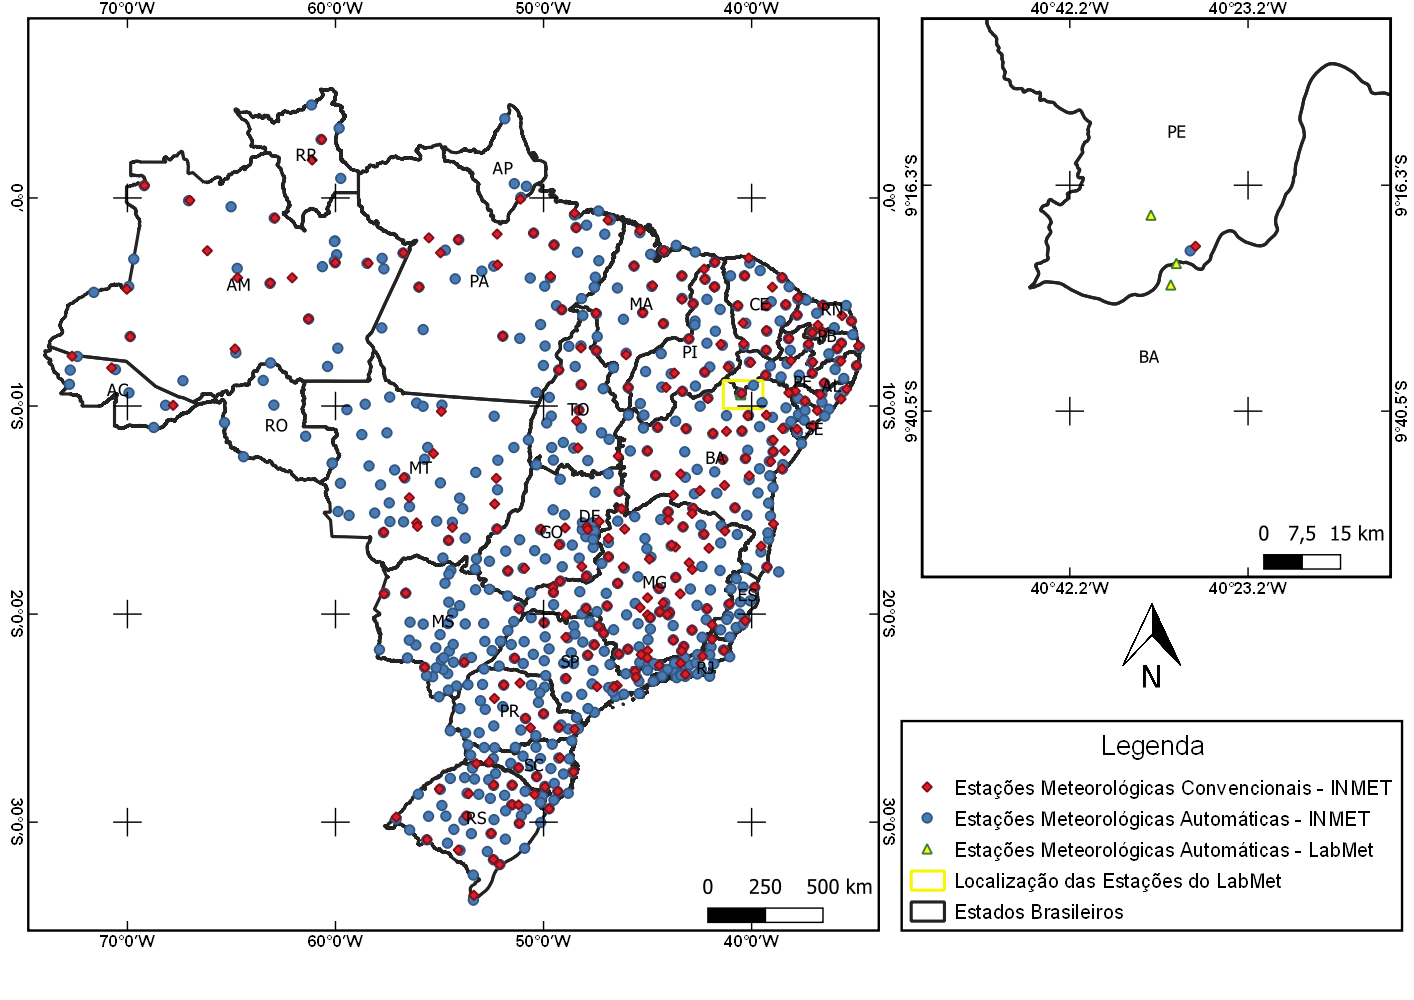
\includegraphics[width=0.8\textwidth]{figuras/espacializacao_estacoes.png}
\end{figure}

\end{columns}

\end{frame}

% ----------------- NOVO SLIDE --------------------------------
\section{Processamento e Tratamento dos Dados}

\begin{frame}{Processamento e Tratamento dos Dados}
\frametitle{Processamento e Tratamento dos Dados}

\begin{itemize}
	\item Conversão dos conjuntos de dados para formato estruturado; 
	\item Conversão dos conjuntos de dados para frequência diária; 
	\item Eliminando valores inconsistentes: inconsistências de limites, inconsistências lógicas e inconsistências temporais.
\end{itemize}

\end{frame}

% ----------------- NOVO SLIDE --------------------------------

\section{Análise e Exploração dos Dados}

\begin{frame}
    \frametitle{Análise e Exploração dos Dados}

	\begin{figure}[H]
	\centering
	\caption{Distribuição, por estado, das estações meteorológicas analisadas.}
	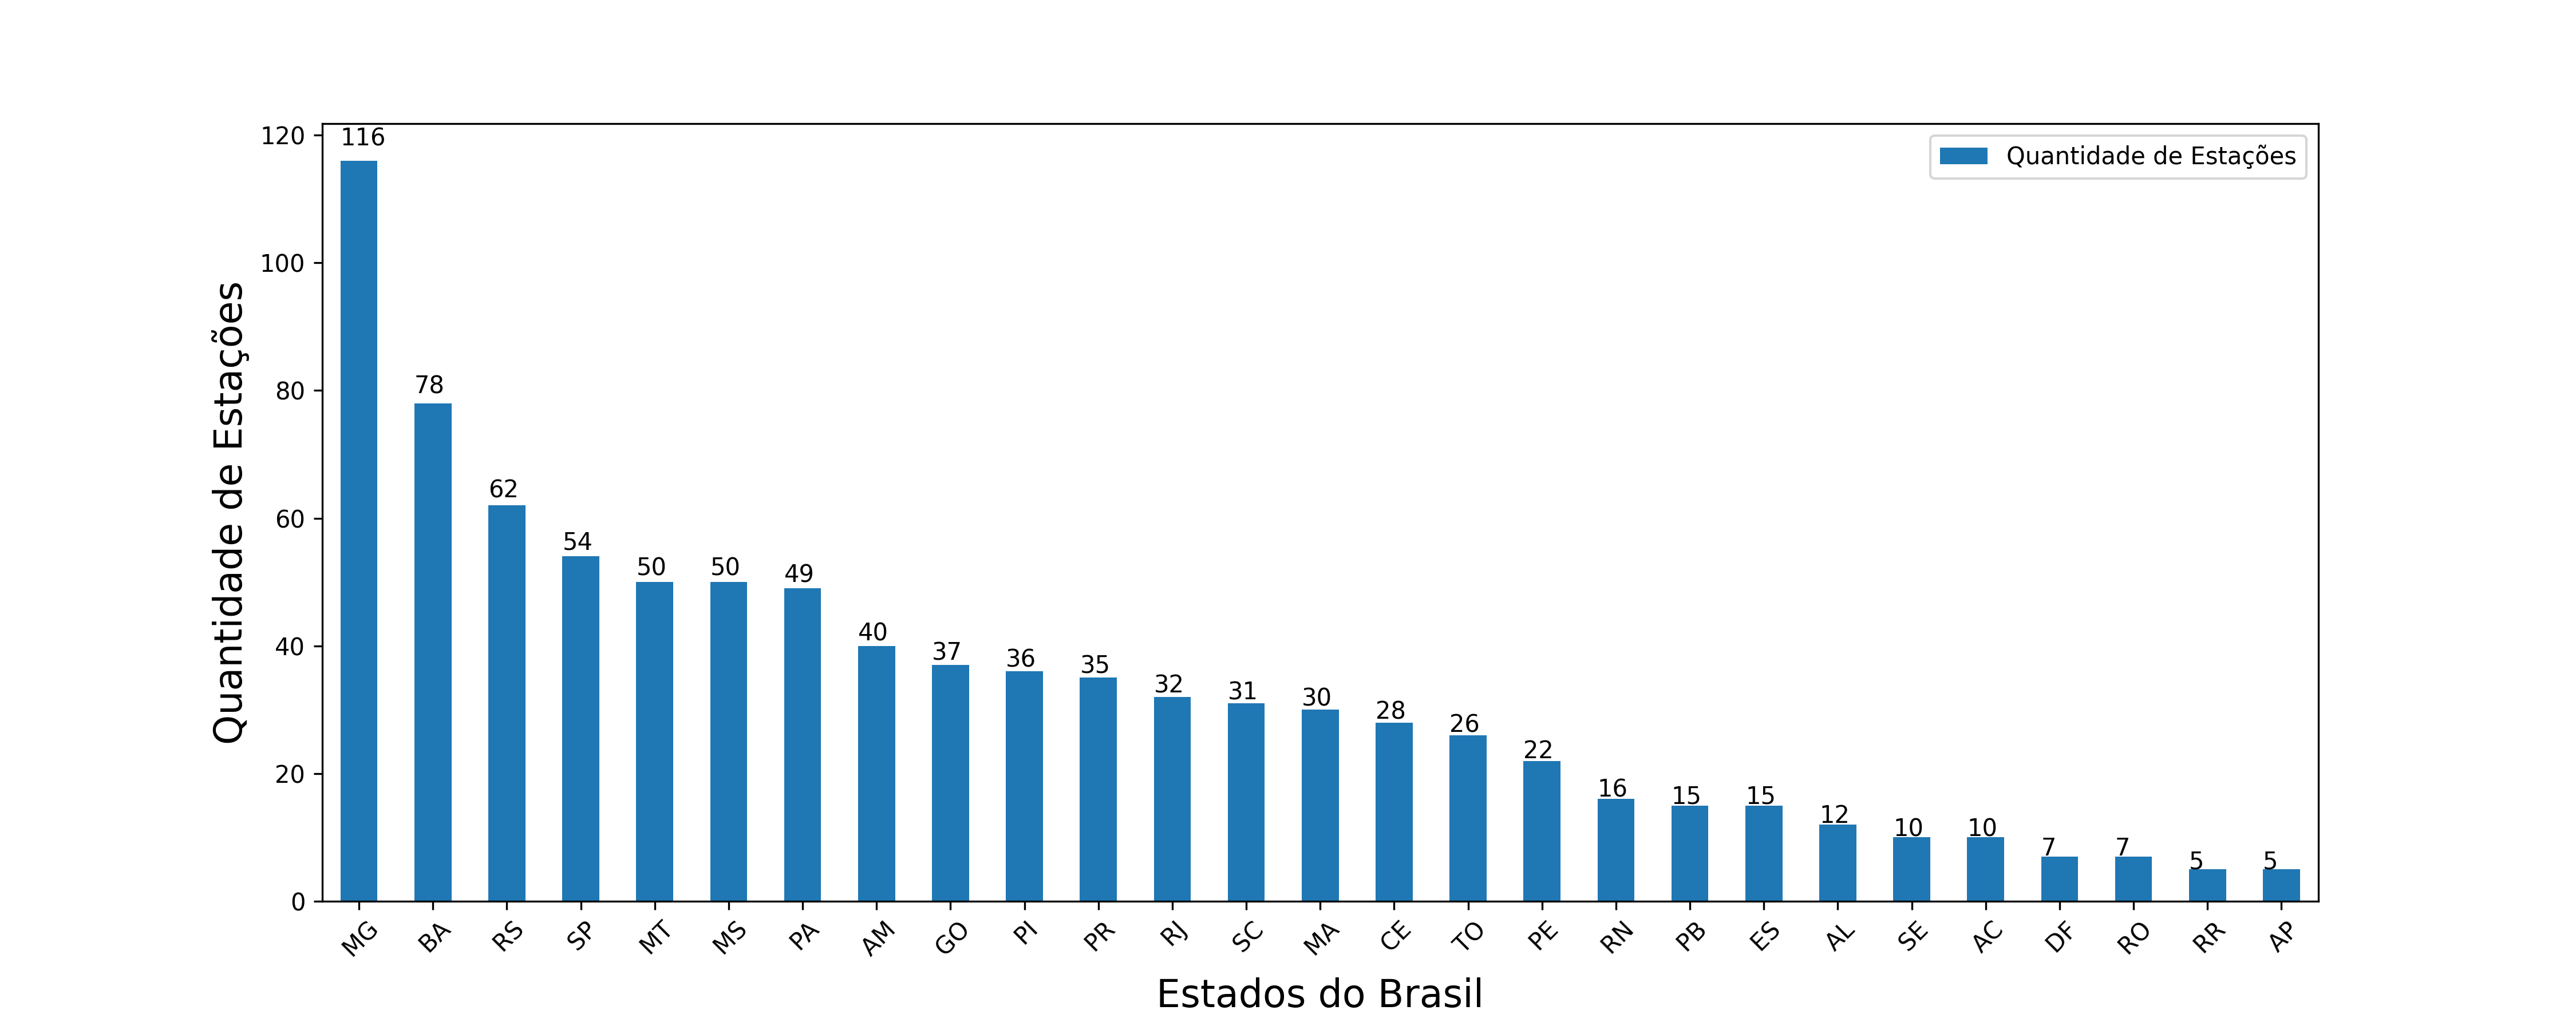
\includegraphics[width=0.8\textwidth]{figuras/estacoes_por_estado.png}
	\end{figure}
\end{frame}

\begin{frame}
    \frametitle{Análise e Exploração dos Dados}

	\begin{figure}[H]
	\centering
	\caption{Quantidade de registros disponíveis ao longo de todo o período analisado.}
	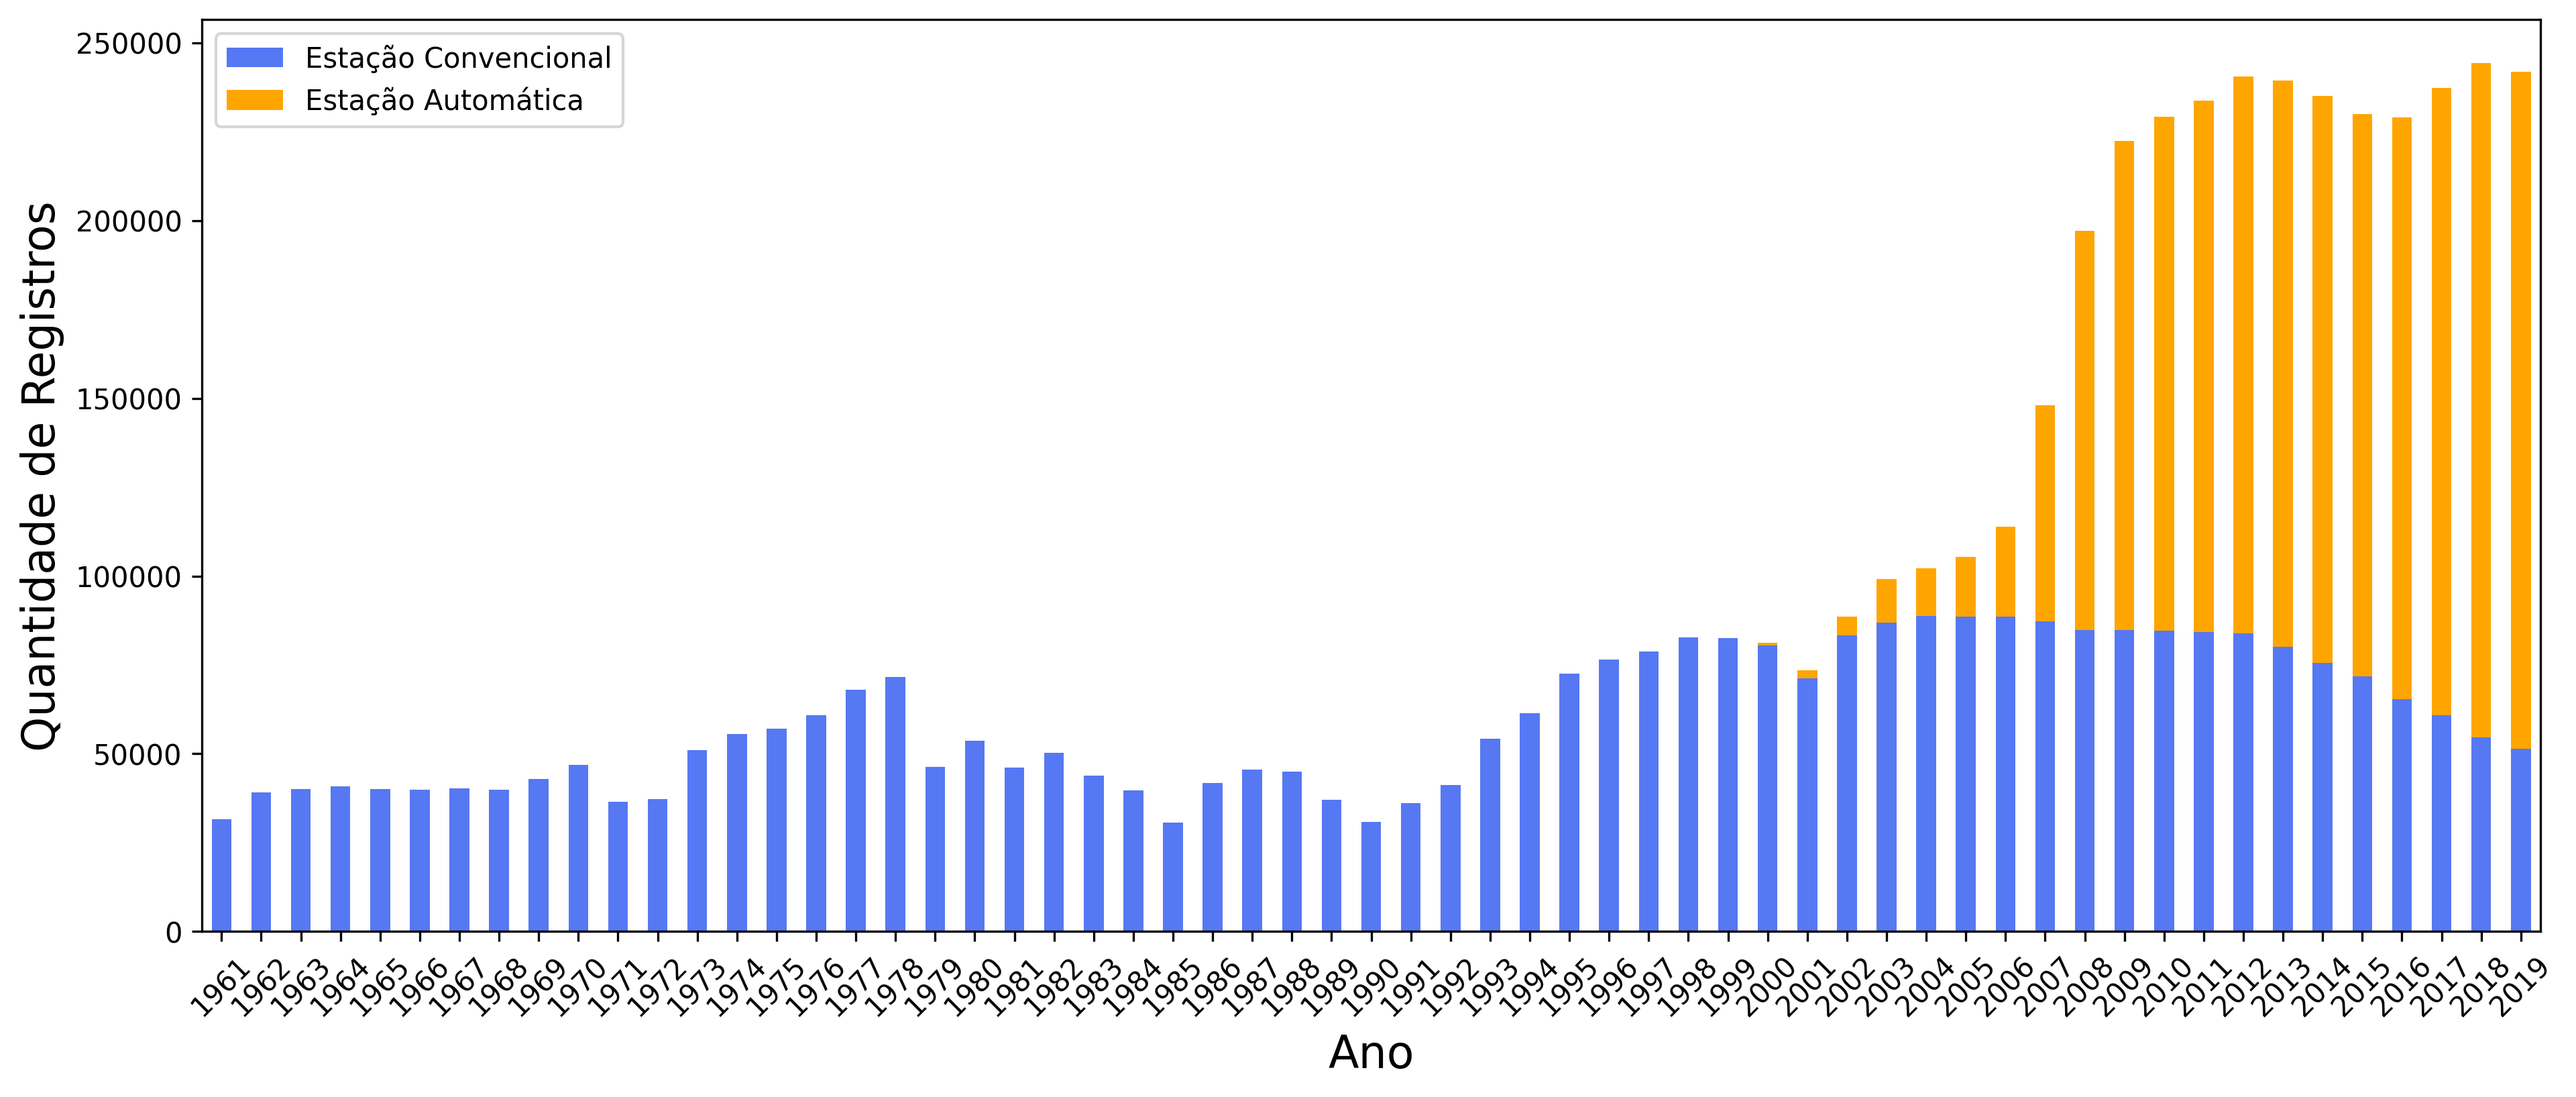
\includegraphics[width=0.8\textwidth]{figuras/disponibilizade_historica_de_dados.png}
	\end{figure}
\end{frame}

\begin{frame}
    \frametitle{Análise e Exploração dos Dados}

	\begin{figure}[H]
	\centering
	\caption{Quantidade de registos disponíveis e nulos ao longo de todo o período analisado.}
	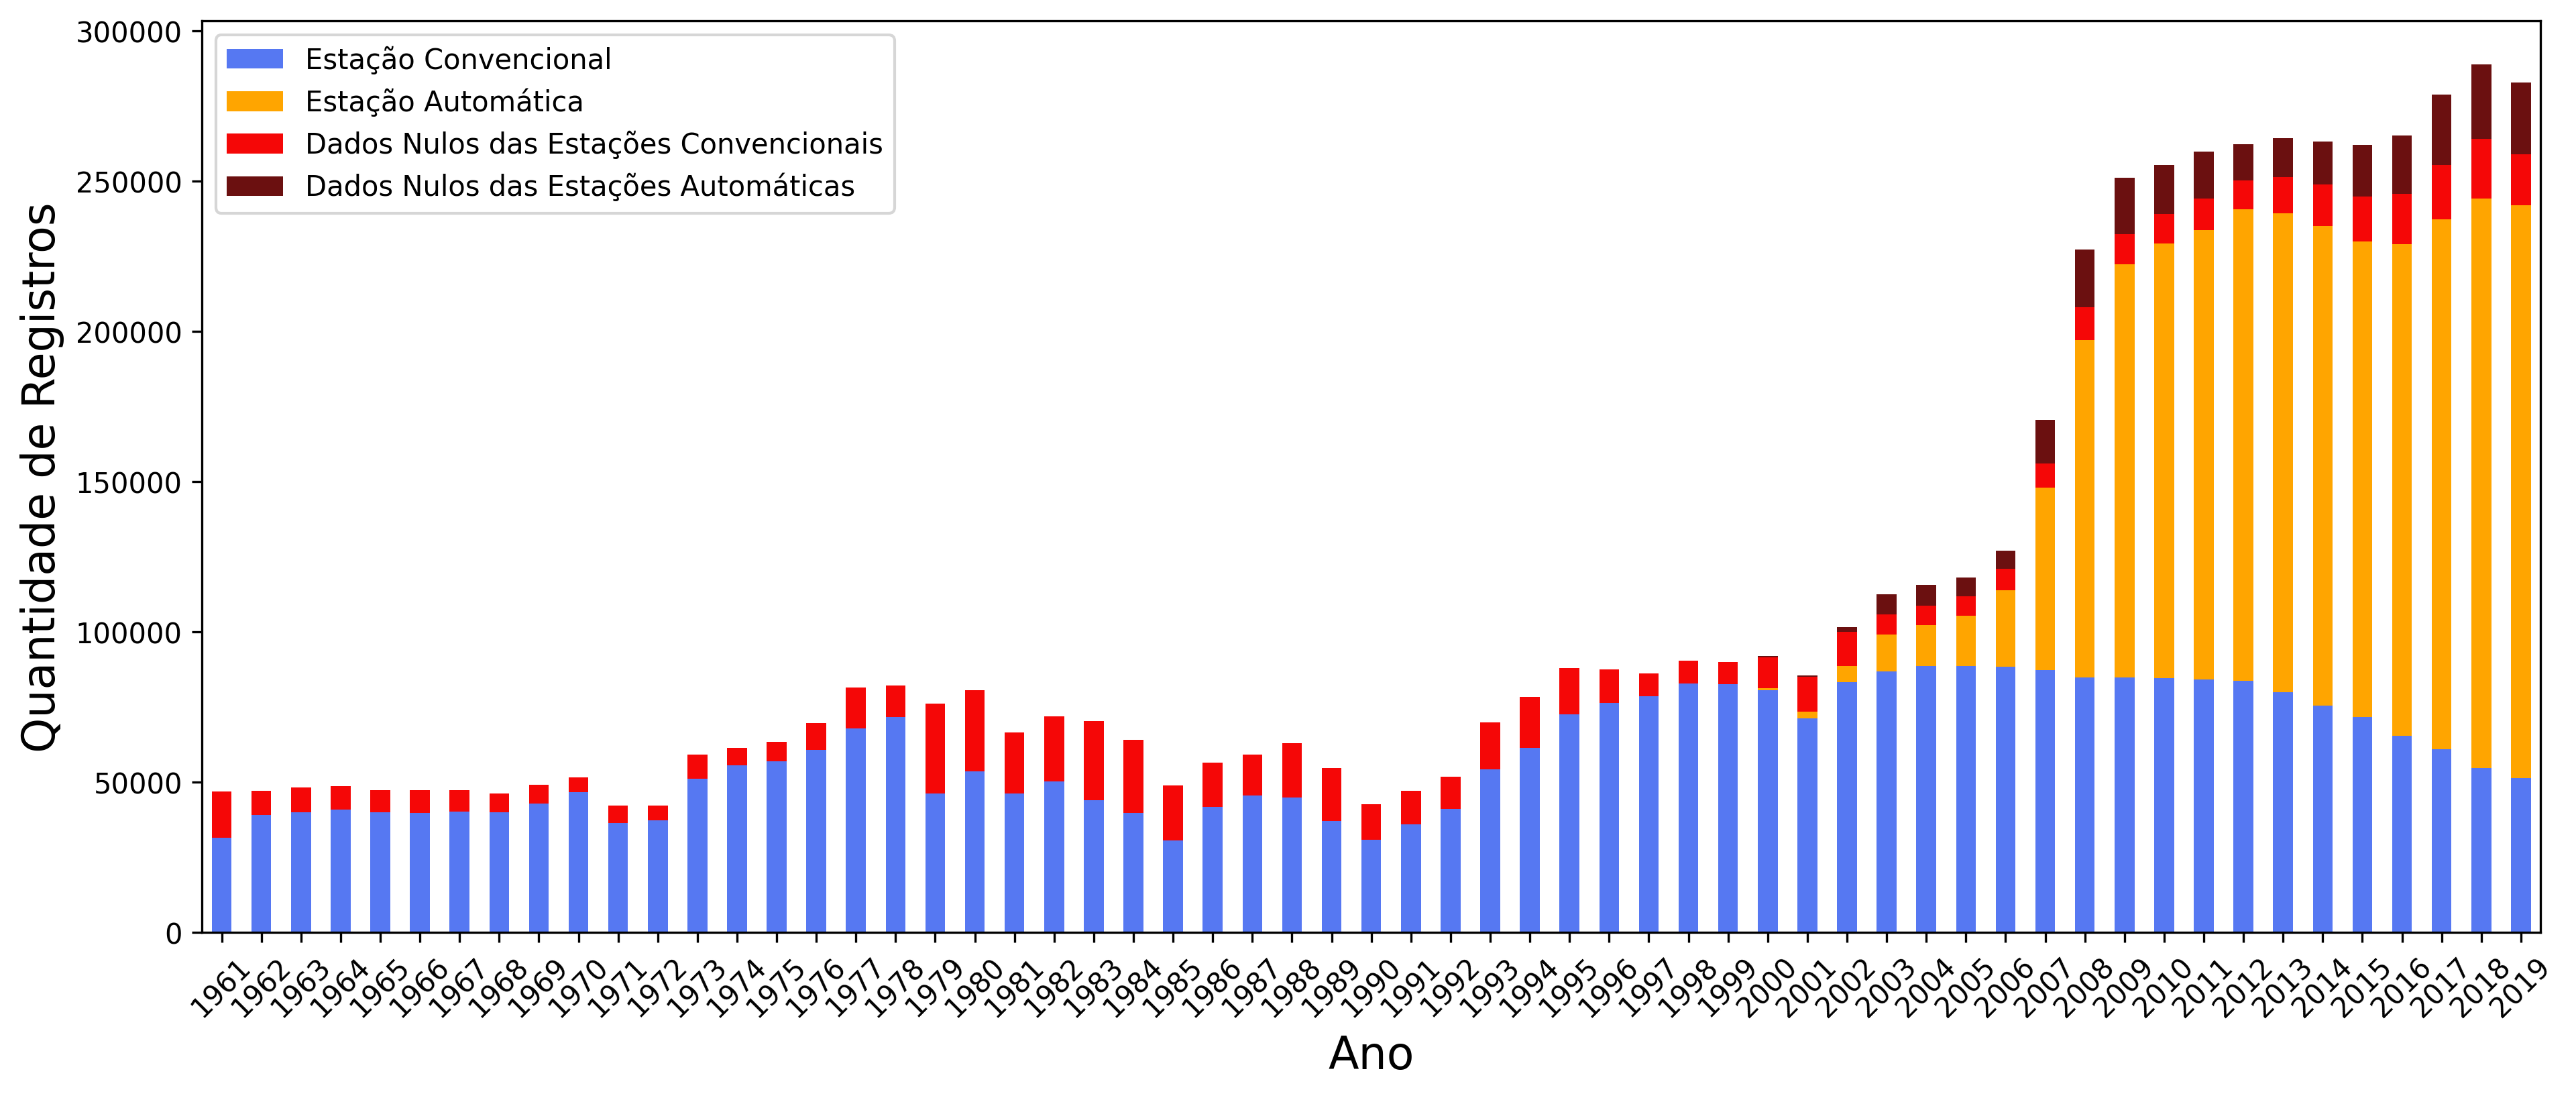
\includegraphics[width=0.8\textwidth]{figuras/dados_ausentes_ao_longo_anos.png}
	\end{figure}
\end{frame}

\begin{frame}
    \frametitle{Análise e Exploração dos Dados}

	\begin{figure}[H]
	\centering
	\caption{Recorde das maiores temperaturas já registradas no período de 1961 a 2019 nas estações convencionais do INMET.}
	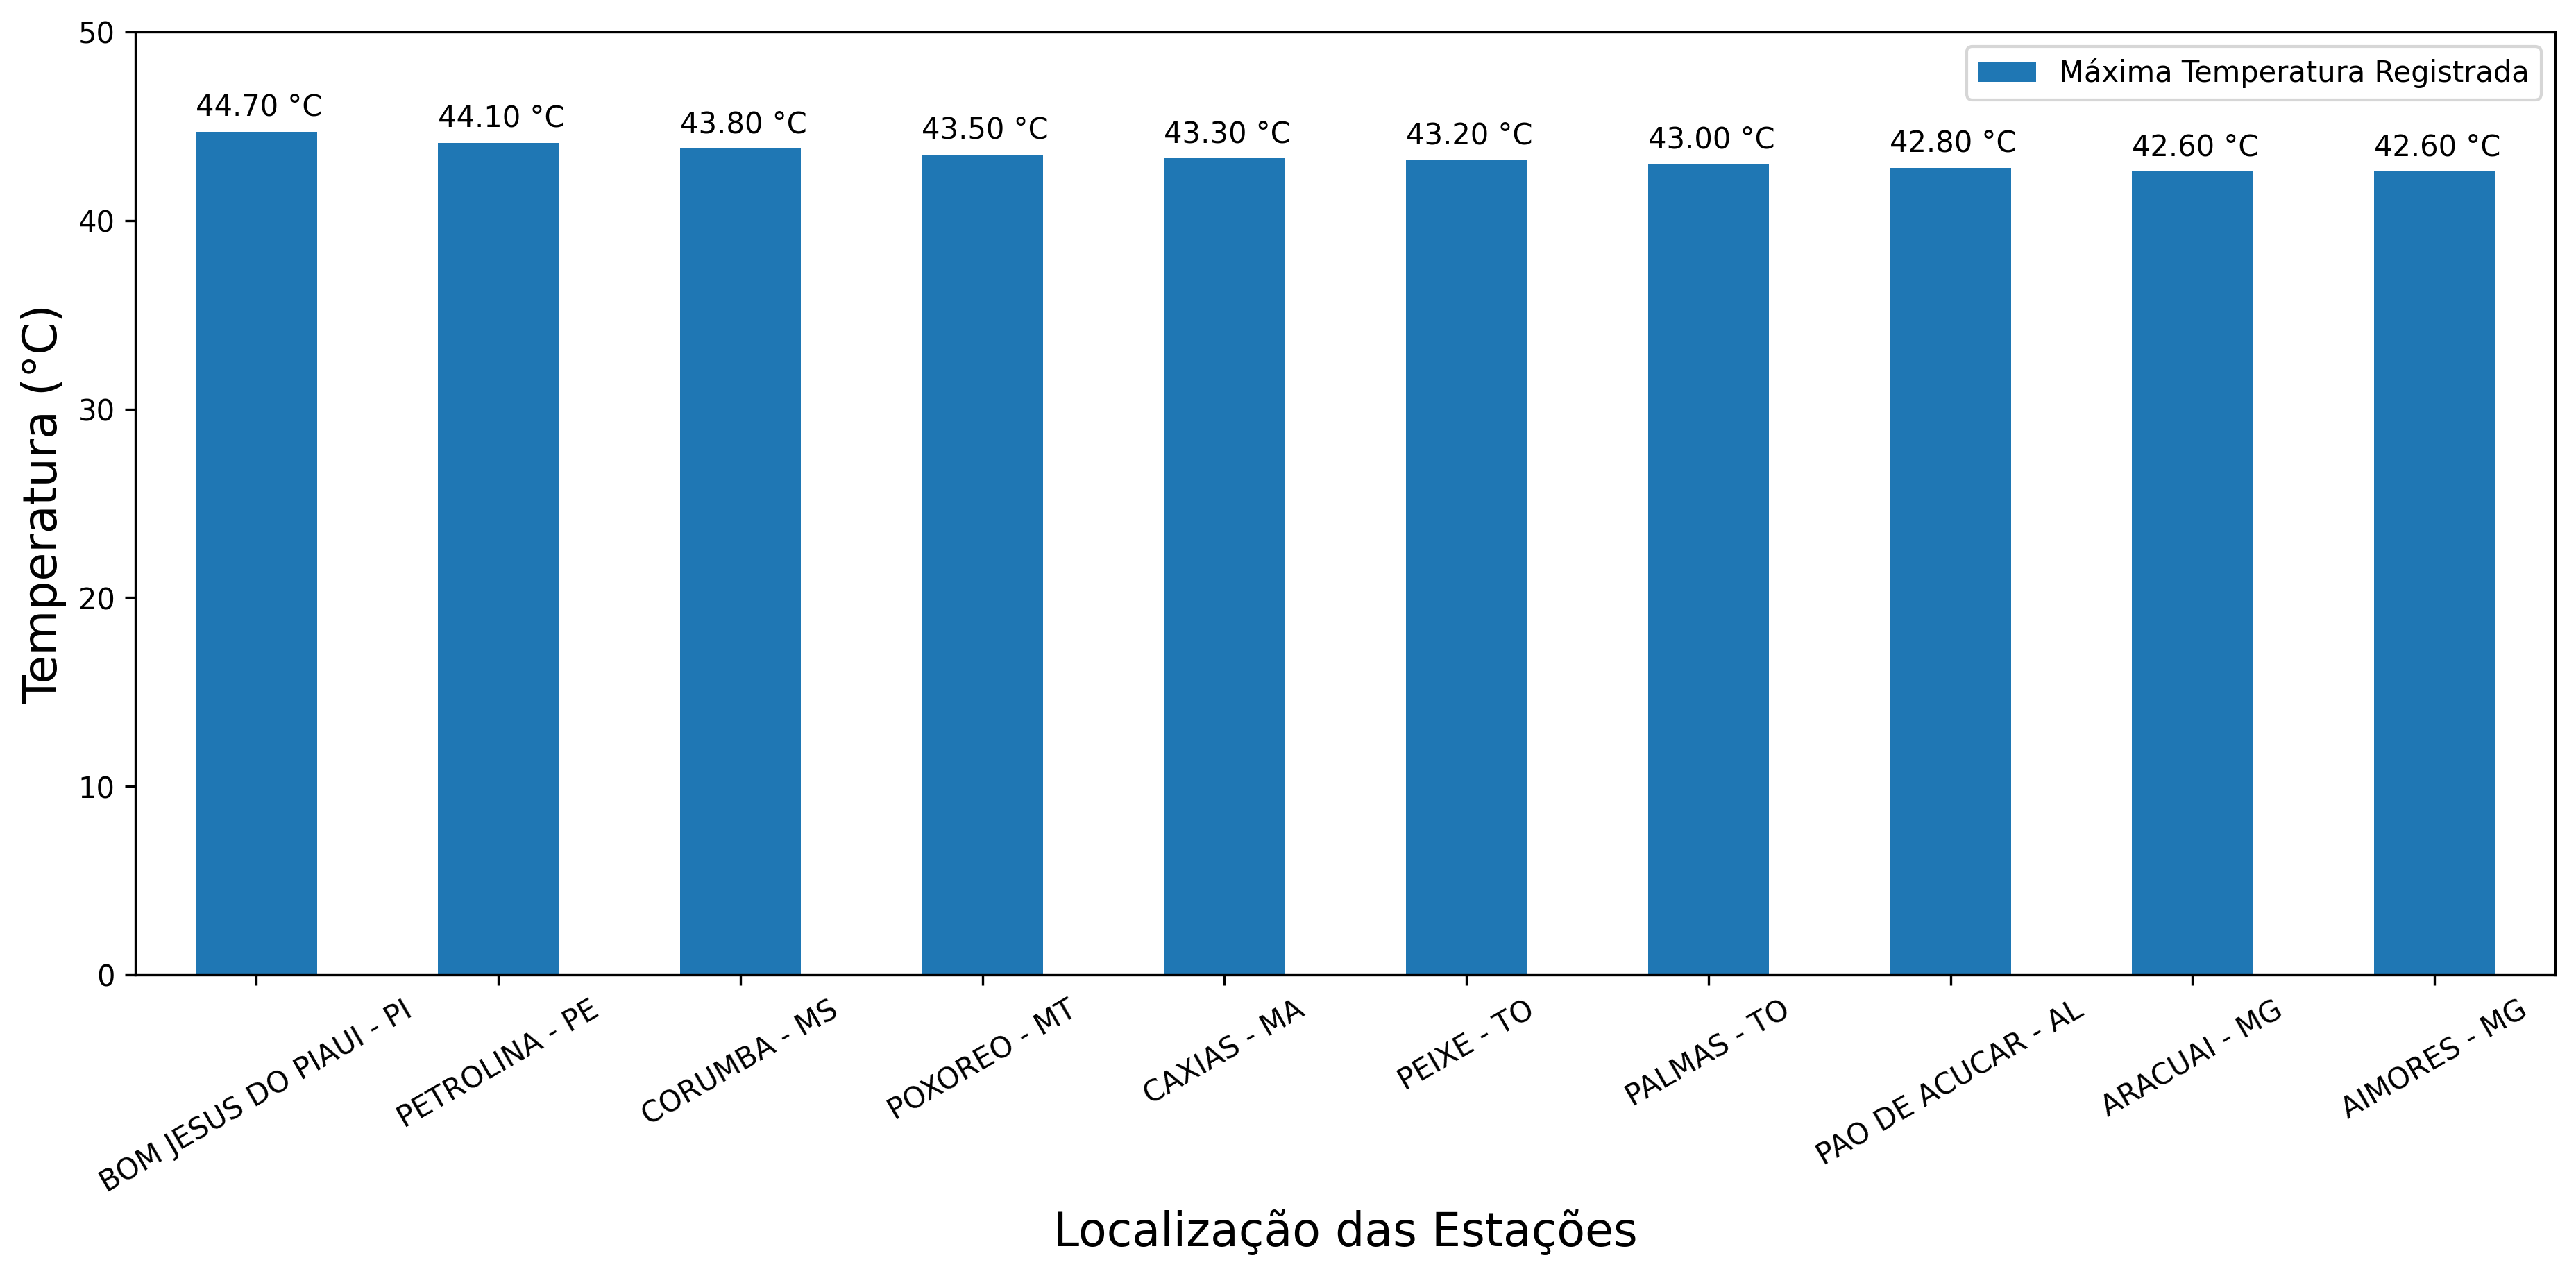
\includegraphics[width=0.8\textwidth]{figuras/estacoes_convencionais_maiores_temperaturas.png}
	\end{figure}
\end{frame}


\begin{frame}
    \frametitle{Análise e Exploração dos Dados}

	\begin{figure}[H]
	\centering
	\caption{Recorde das menores temperaturas já registradas no período de 1961 a 2019 nas estações convencionais do INMET.}
	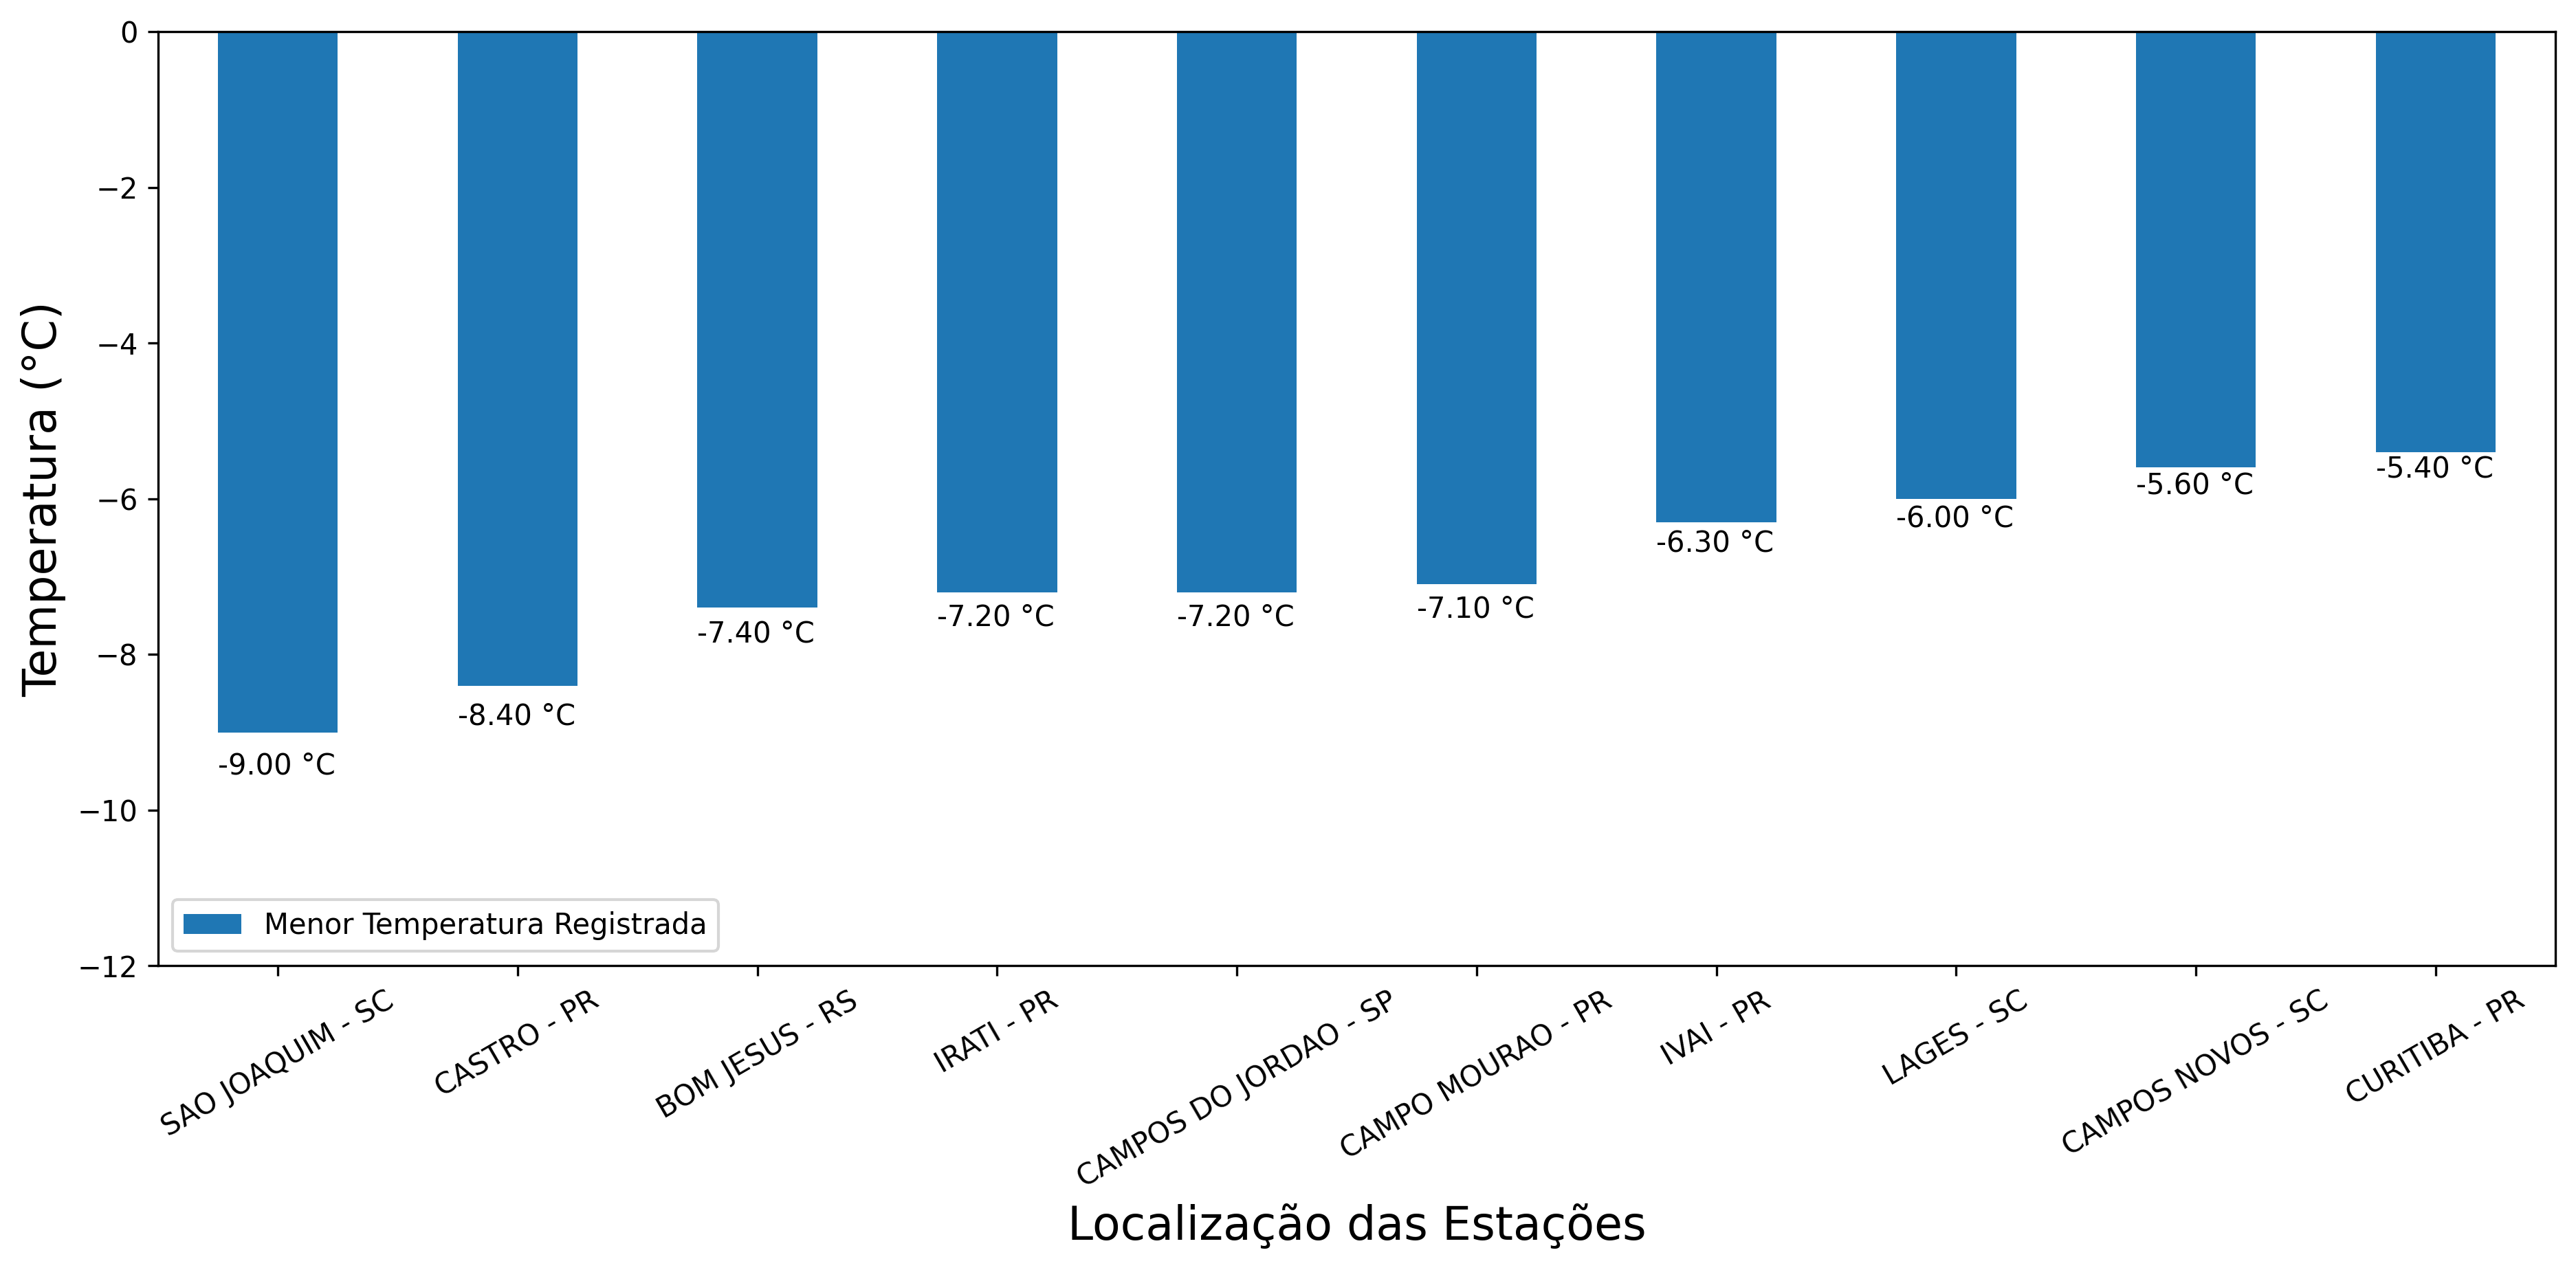
\includegraphics[width=0.8\textwidth]{figuras/estacoes_convencionais_menores_temperaturas.png}
	\end{figure}
\end{frame}

% ----------------- NOVO SLIDE --------------------------------

\section{Criação dos Modelos de Aprendizado de Máquina}

\begin{frame}
\frametitle{Criação dos Modelos de Aprendizado de Máquina}

\begin{columns}
\column{0.5\textwidth}

\begin{figure}[H]
\centering
\caption{Autoregressive integrated moving average (ARIMA).}

\includegraphics[width=0.35\textwidth]{figuras/arima.png}
\end{figure}

\column{0.5\textwidth}

\begin{figure}[H]
\centering
\caption{Long Short-Term Memory (LSTM).}
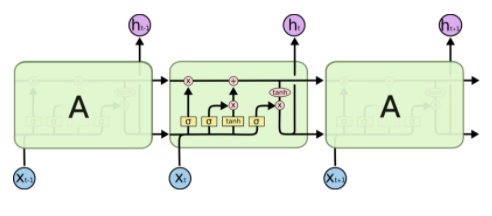
\includegraphics[width=0.8\textwidth]{figuras/lstm.png}
\end{figure}

\end{columns}

\end{frame}


\begin{frame}
\frametitle{Modelo ARIMA}

\begin{figure}[H]
\centering
\caption{Exemplo da decomposição de uma série temporal.}
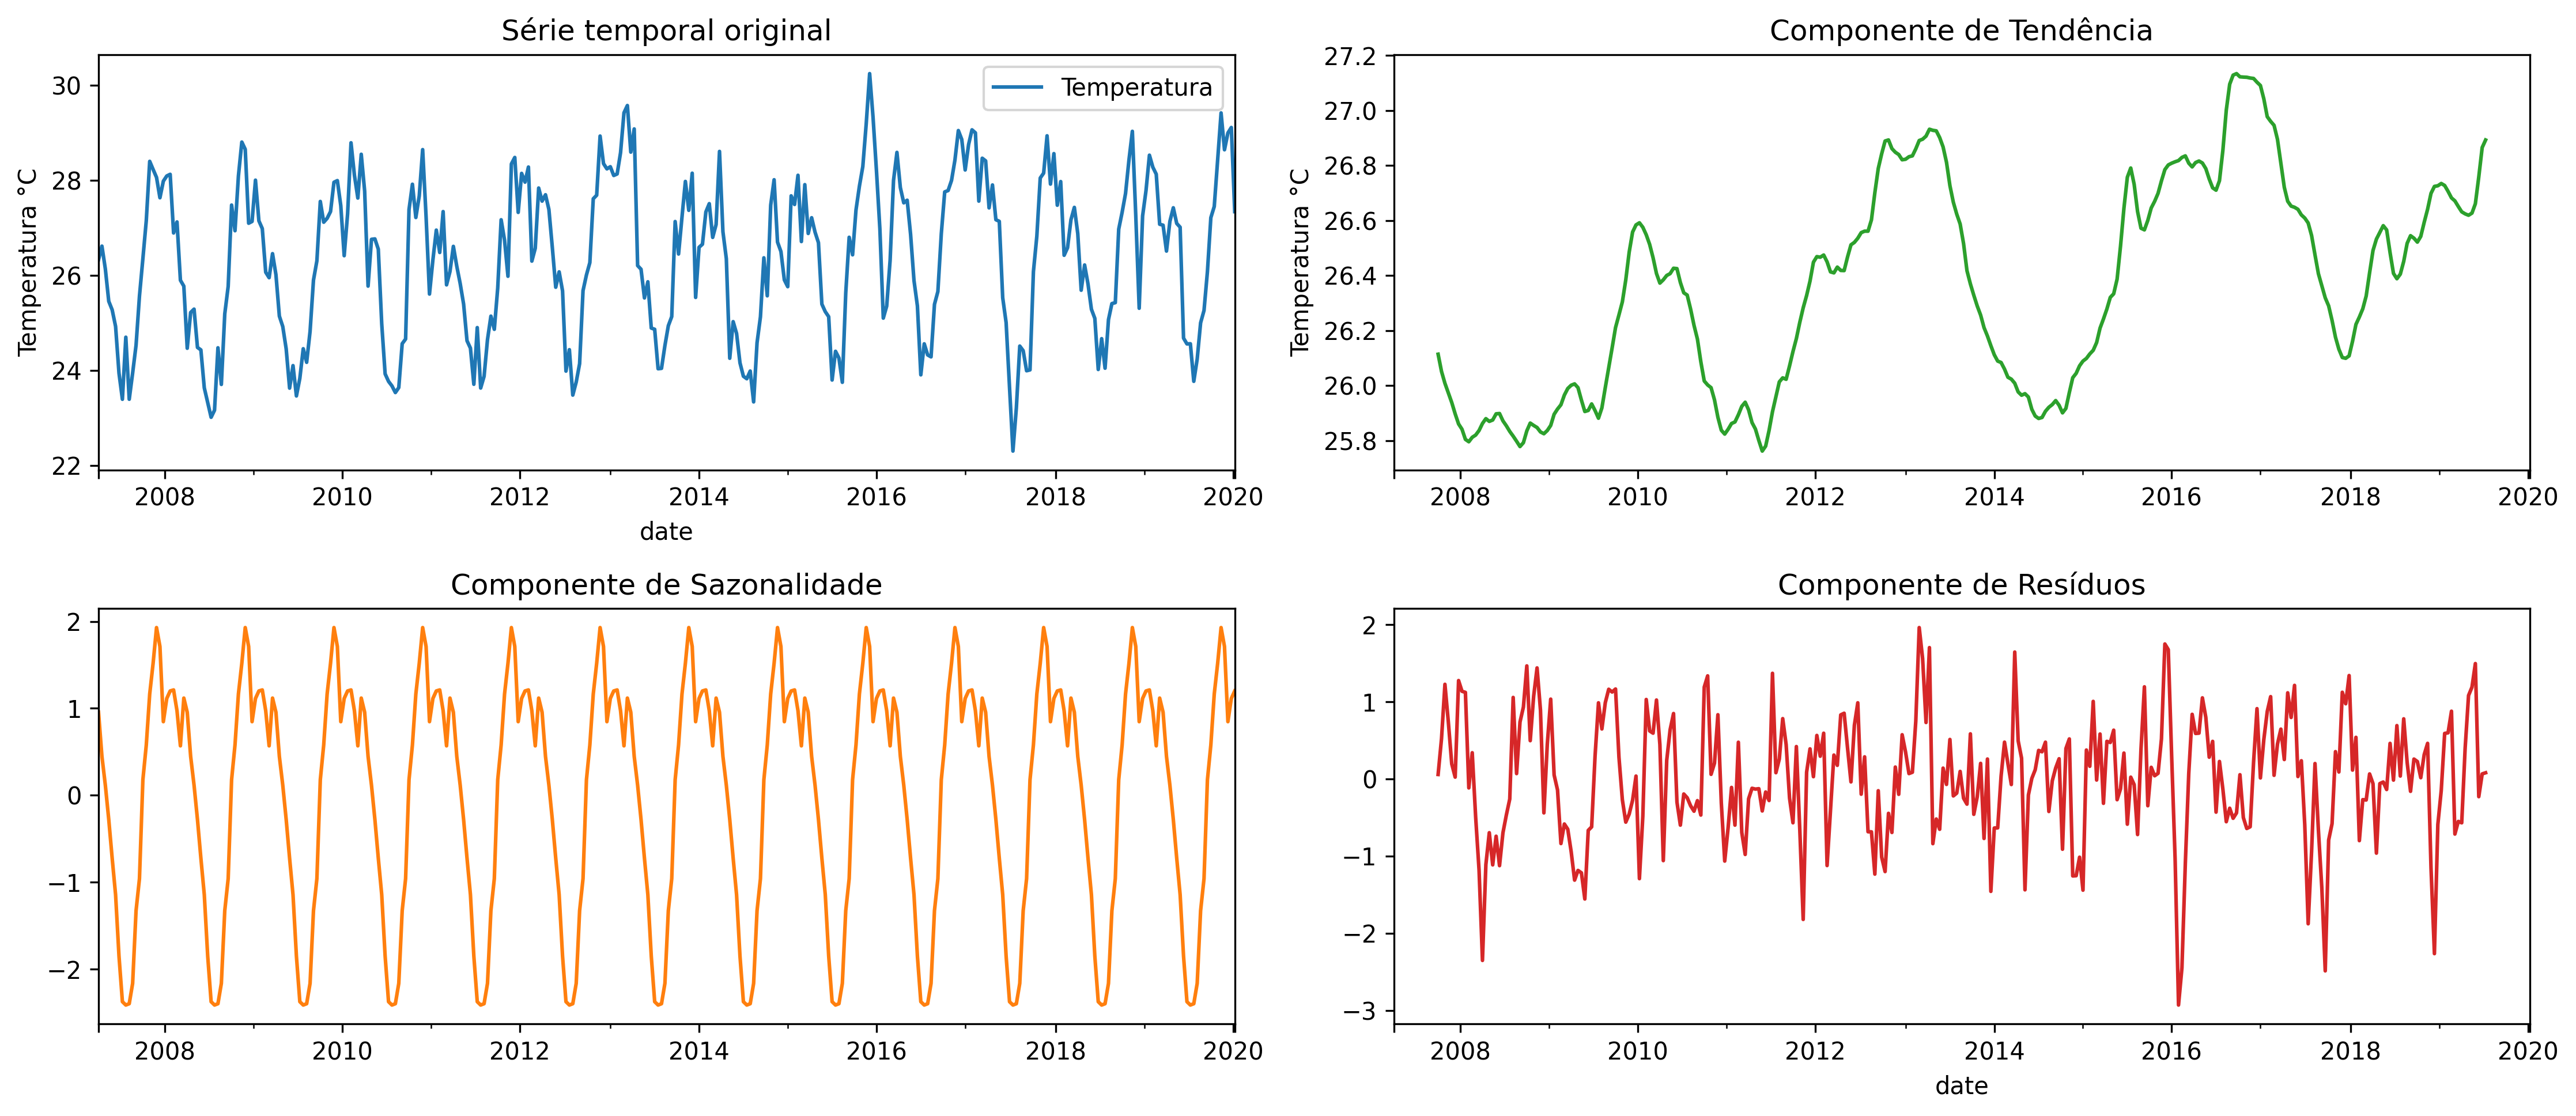
\includegraphics[width=0.8\textwidth]{figuras/decomposicao_712f3e11658051636f09732a60fb3c1b.png}
\end{figure}

\end{frame}

\begin{frame}
\frametitle{Modelo ARIMA}

\begin{figure}[H]
\centering
\caption{Exemplo de autocorrelação para uma série temporal.}
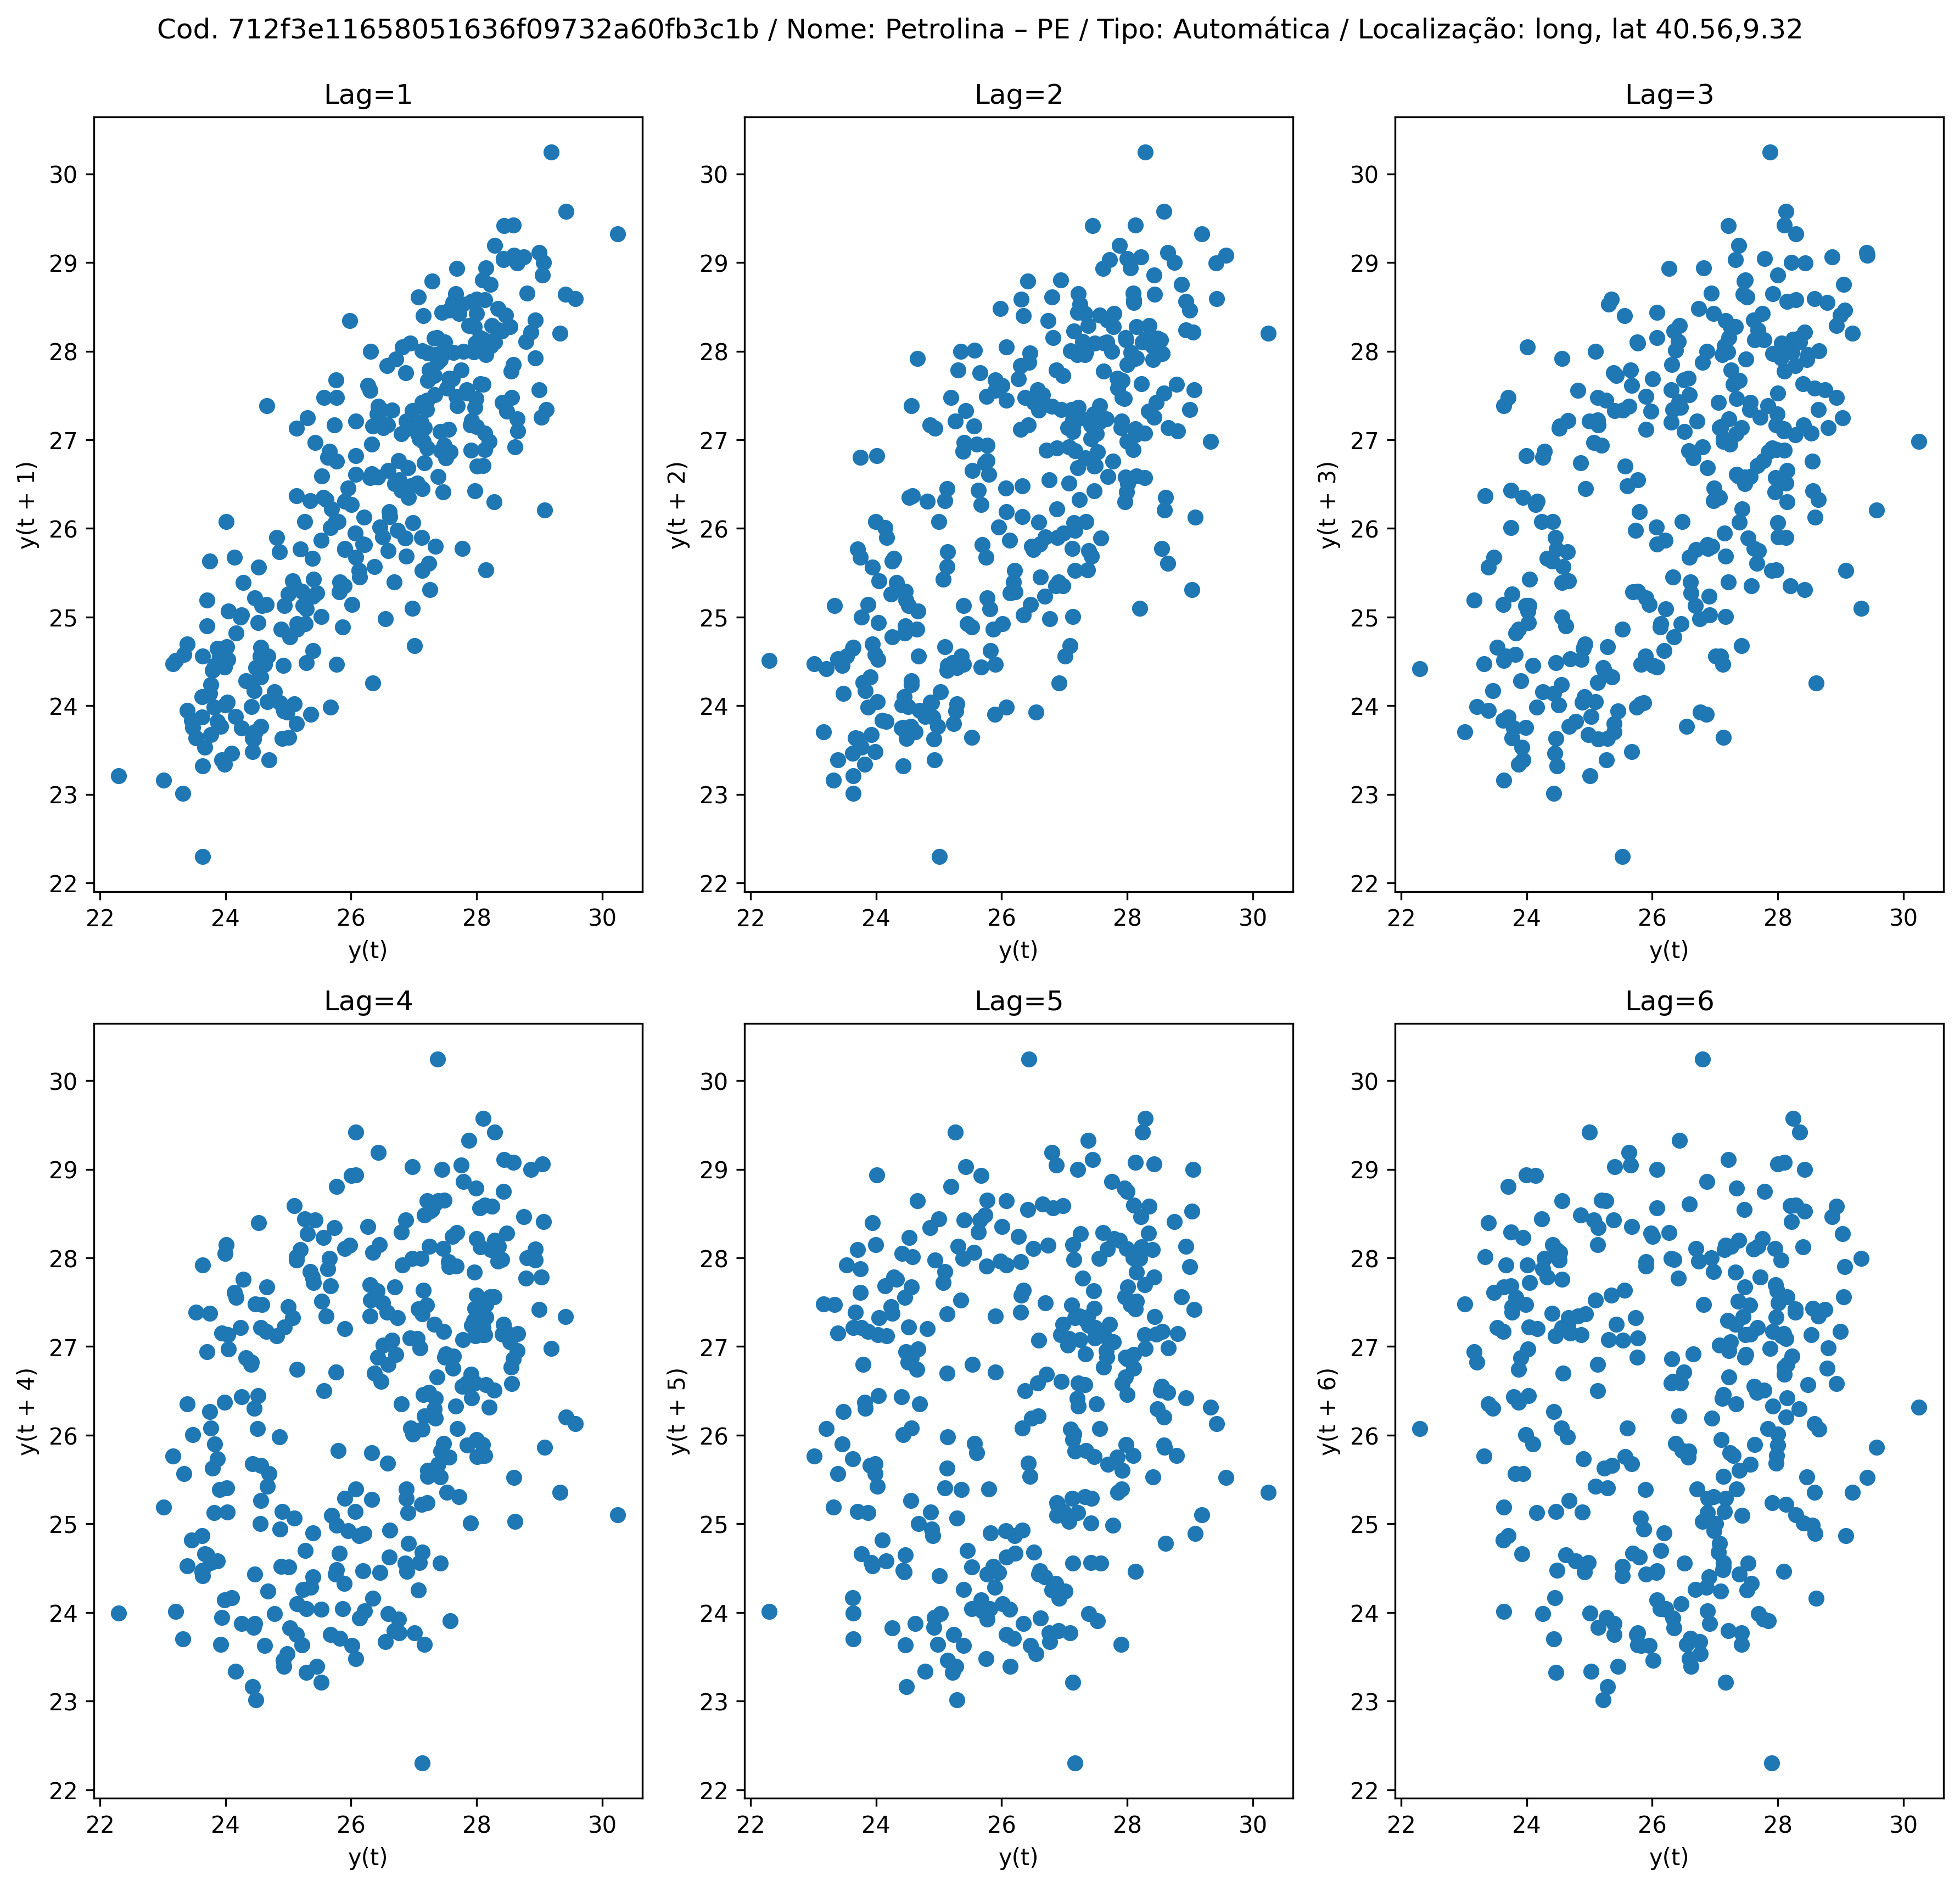
\includegraphics[width=0.4\textwidth]{figuras/correlacao_712f3e11658051636f09732a60fb3c1b.png}
\end{figure}

\end{frame}

\begin{frame}
\frametitle{Modelo ARIMA}

\begin{figure}[H]
\centering
\caption{Exemplo de teste de estacionariedade à série temporal original.}
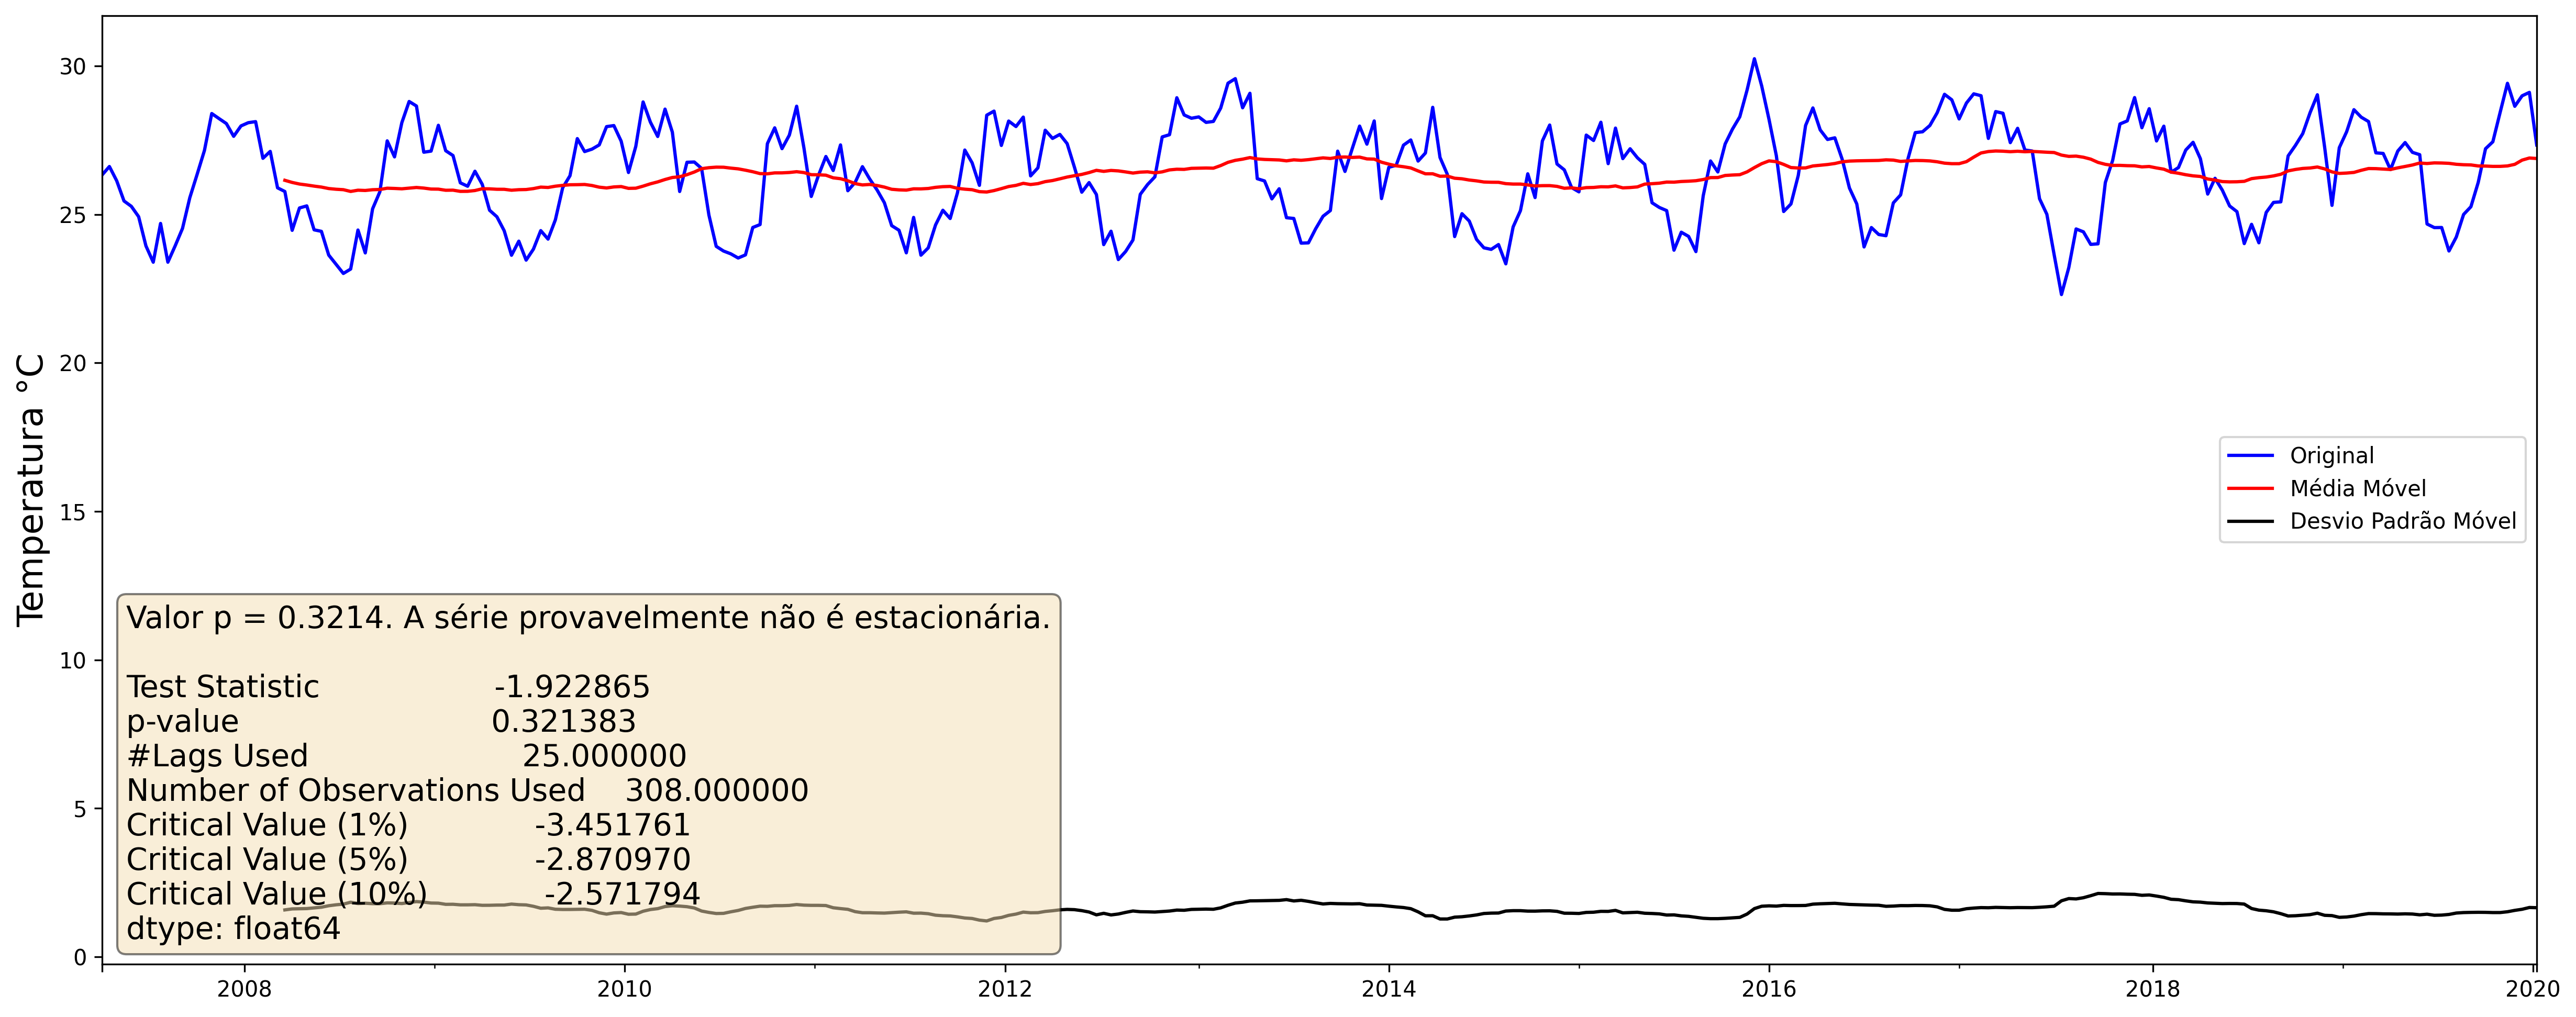
\includegraphics[width=0.8\textwidth]{figuras/dickey_fuller_raw_712f3e11658051636f09732a60fb3c1b.png}
\end{figure}

\end{frame}

\begin{frame}
\frametitle{Modelo ARIMA}

\begin{figure}[H]
\centering
\caption{Exemplo de teste de estacionariedade aplicado à série temporal diferenciada.}
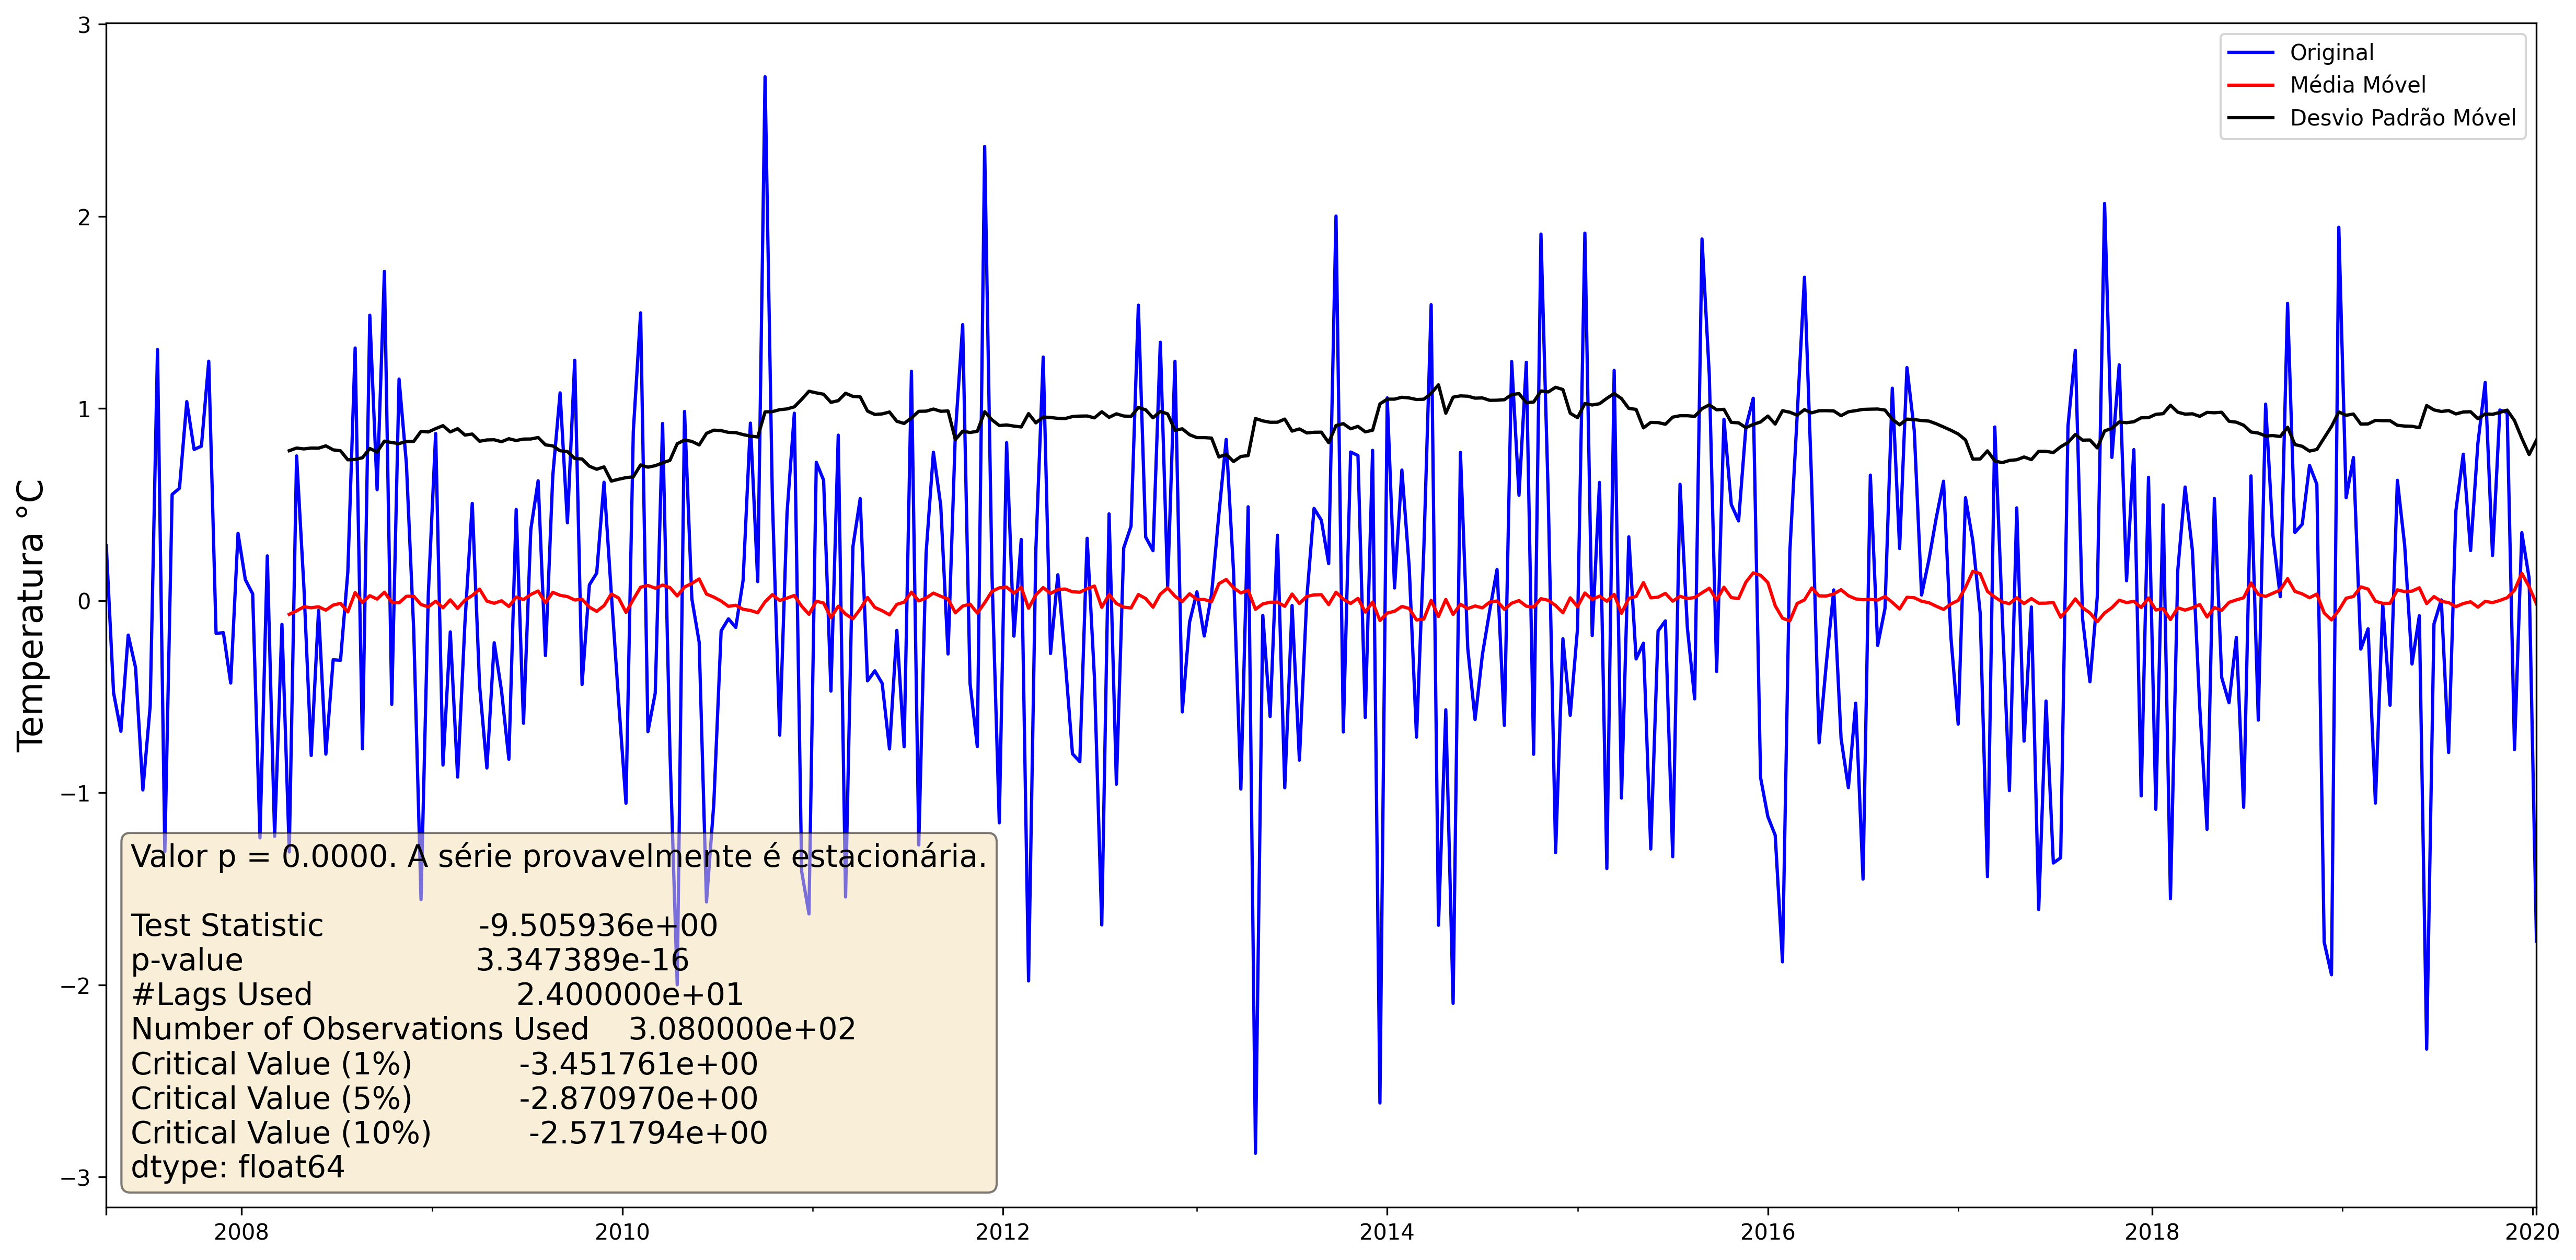
\includegraphics[width=0.8\textwidth]{figuras/dickey_fuller_diff_712f3e11658051636f09732a60fb3c1b.png}
\end{figure}

\end{frame}


\begin{frame}
\frametitle{Modelo ARIMA}

\begin{figure}[H]
\centering
\caption{Parametrização do modelo auto arima e predição do ano de 2019 para as 88 séries temporais selecionadas de teste.}
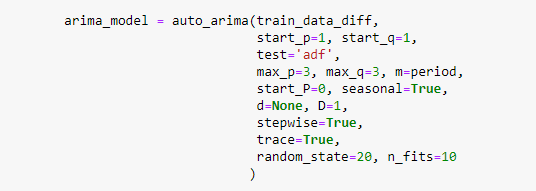
\includegraphics[width=0.8\textwidth]{figuras/parametros_autoarima.png}
\end{figure}

\end{frame}

% ----------------- NOVO SLIDE --------------------------------

\begin{frame}
\frametitle{Model LSTM}

\begin{columns}
\column{0.5\textwidth}

\resizebox{\textwidth}{!}{
\begin{tabular}{|c|c|}
\hline
\textbf{Período para obter o dado de entrada (X)} & \textbf{Período para obter a saída esperada (Y)}\\
\hline
todos os dados anteriores à 01/01/2019  & 01/01/2019 - 31/12/2019 \\
\hline
todos os dados anteriores à 01/01/2018  & 01/01/2018 - 31/12/2018 \\
\hline
---  & --- - ---  \\
\hline
todos os dados anteriores à 01/01/2010  & 01/01/2010 - 31/12/2010 \\
\hline
\end{tabular}
}

\column{0.5\textwidth}

\begin{figure}[H]
\centering
\caption{Dados de Treinamento, Validação e Teste.}
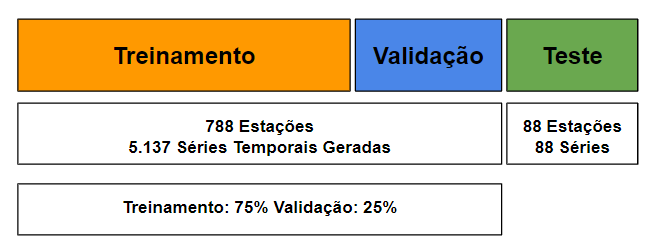
\includegraphics[width=0.8\textwidth]{figuras/conjuntos_treinamento.png}
\end{figure}


\end{columns}

\end{frame}


\begin{frame}
\frametitle{Model LSTM}

\begin{figure}[H]
\centering
\caption{Arquitetura LSTM desenvolvida.}
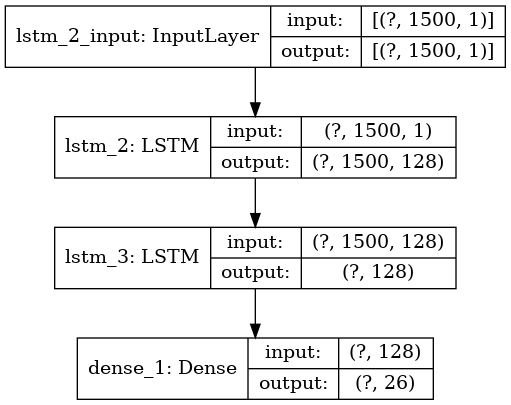
\includegraphics[width=0.3\textwidth]{figuras/lstm_model.png}
\end{figure}

\end{frame}


\begin{frame}
\frametitle{Model LSTM}

\begin{figure}[H]
\centering
\caption{Treinamento do Modelo.}
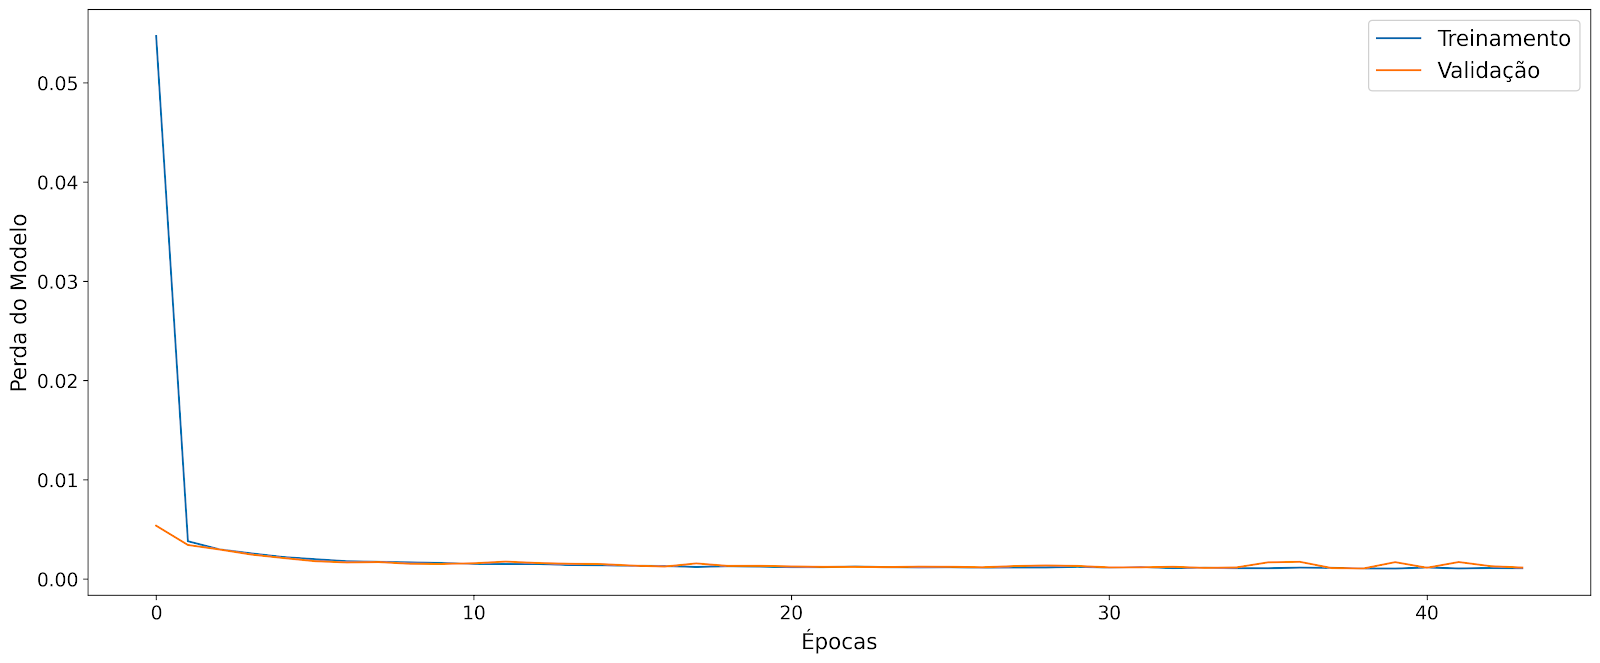
\includegraphics[width=0.9\textwidth]{figuras/lstm_perda_modelo.png}
\end{figure}

\end{frame}


\section{Apresentação dos Resultados}

\begin{frame}
\frametitle{Apresentação dos Resultados}

\begin{figure}[H]
\centering
\caption{Resultado da previsão da temperatura do ar para o ano de 2019 na estação meteorológica localizada no município de Alegrete, no estado do Rio Grande do Sul.}
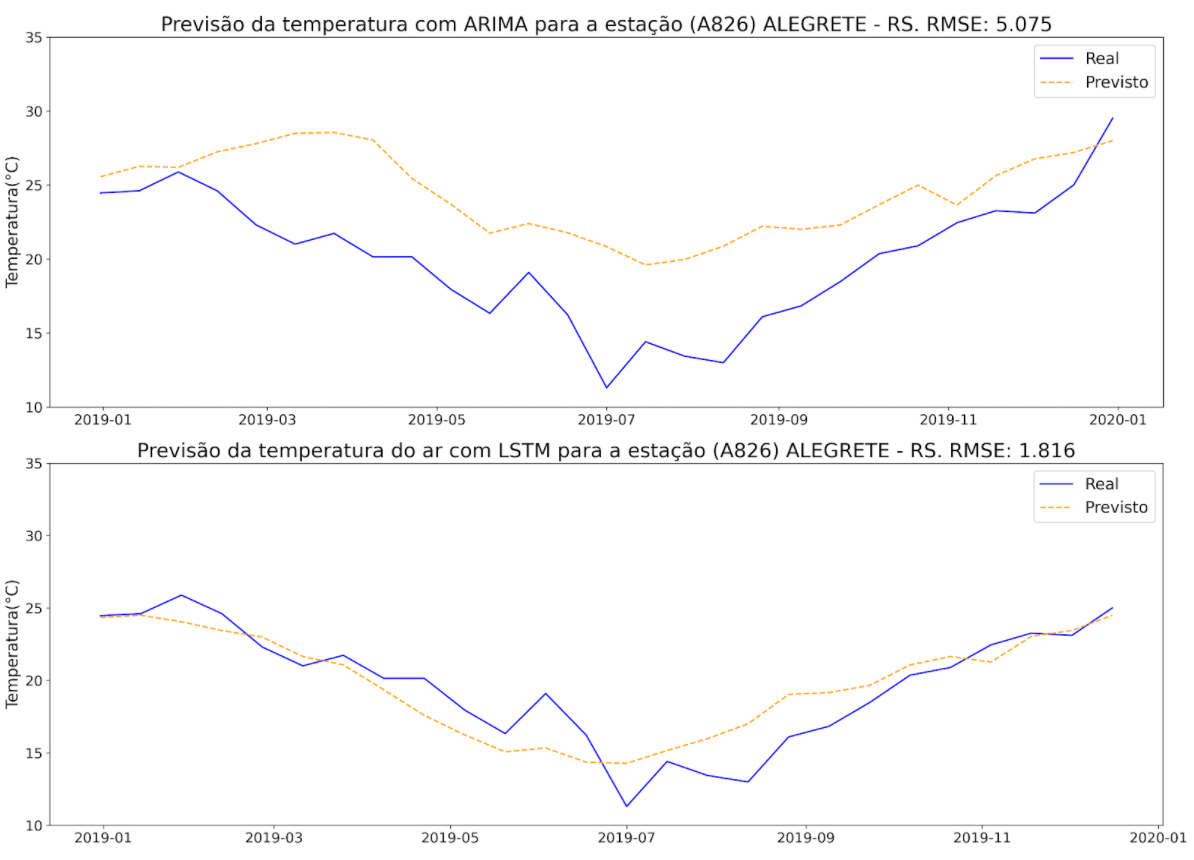
\includegraphics[width=0.5\textwidth]{figuras/resultados_1.png}
\end{figure}

\end{frame}

\begin{frame}
\frametitle{Apresentação dos Resultados}

\begin{figure}[H]
\centering
\caption{Resultado da previsão da temperatura do ar para o ano de 2019 na estação meteorológica localizada no município de Coxim, no estado do Mato Grosso do Sul.}
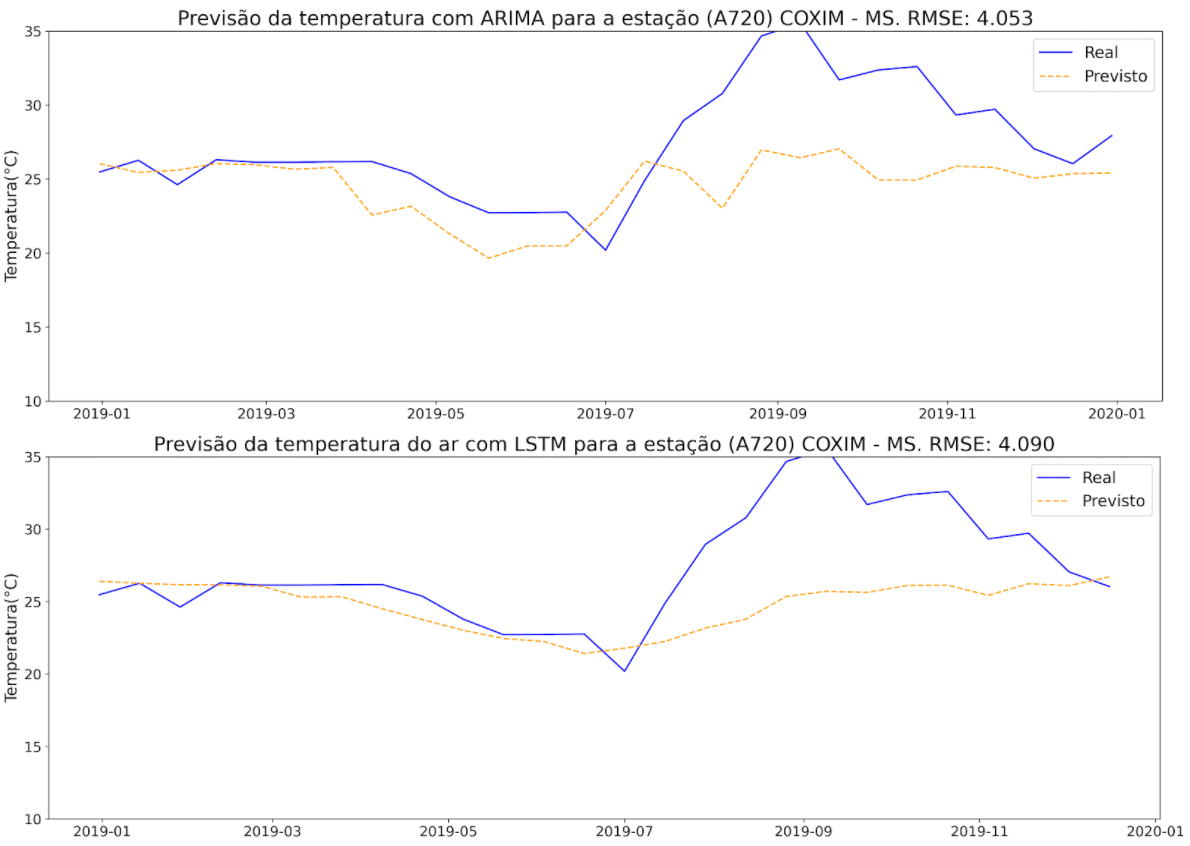
\includegraphics[width=0.5\textwidth]{figuras/resultados_2.png}
\end{figure}

\end{frame}


\begin{frame}
\frametitle{Apresentação dos Resultados}

\begin{figure}[H]
\centering
\caption{Resultado da previsão da temperatura do ar para o ano de 2019 na estação meteorológica localizada no município de Jataí, no estado de Goiás.}
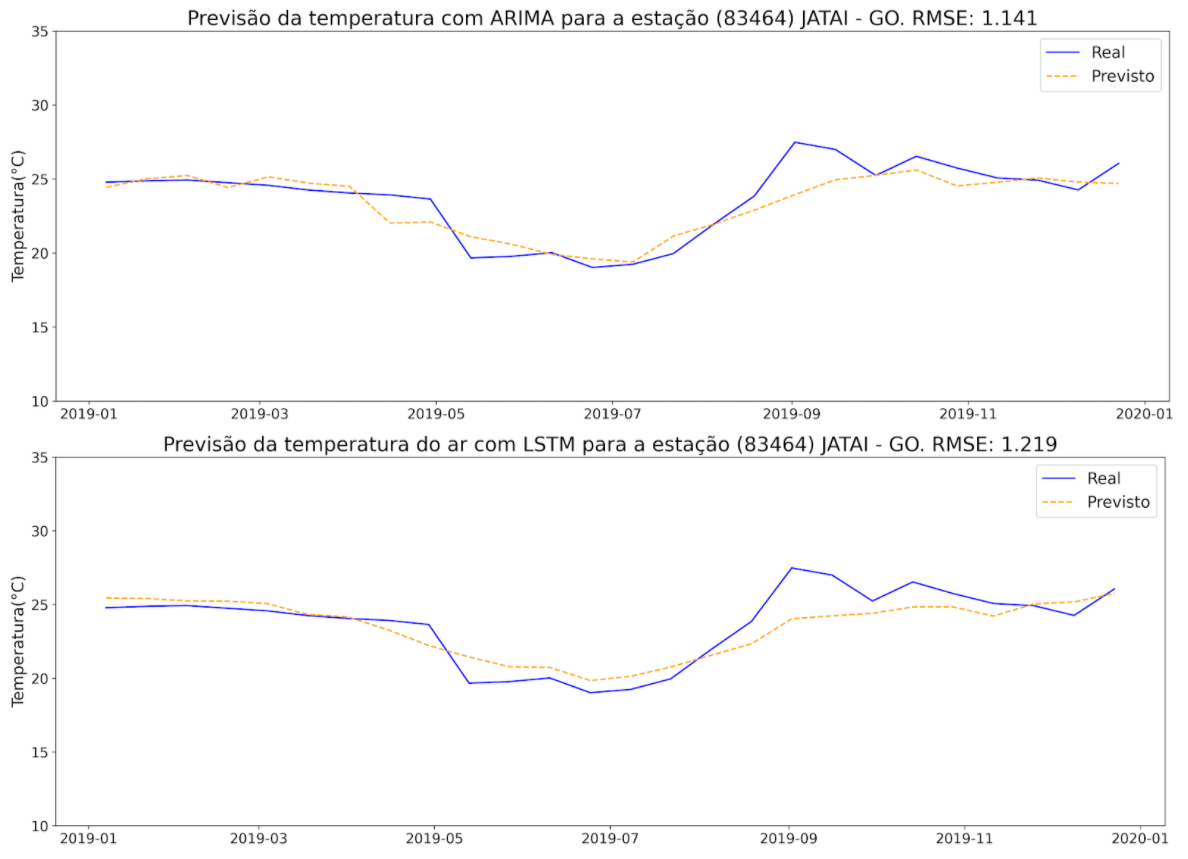
\includegraphics[width=0.5\textwidth]{figuras/resultados_3.png}
\end{figure}

\end{frame}

\begin{frame}
\frametitle{Apresentação dos Resultados}

\begin{figure}[H]
\centering
\caption{Comparação entre os valores obtidos de RMSE para as 88 estações avaliadas.}
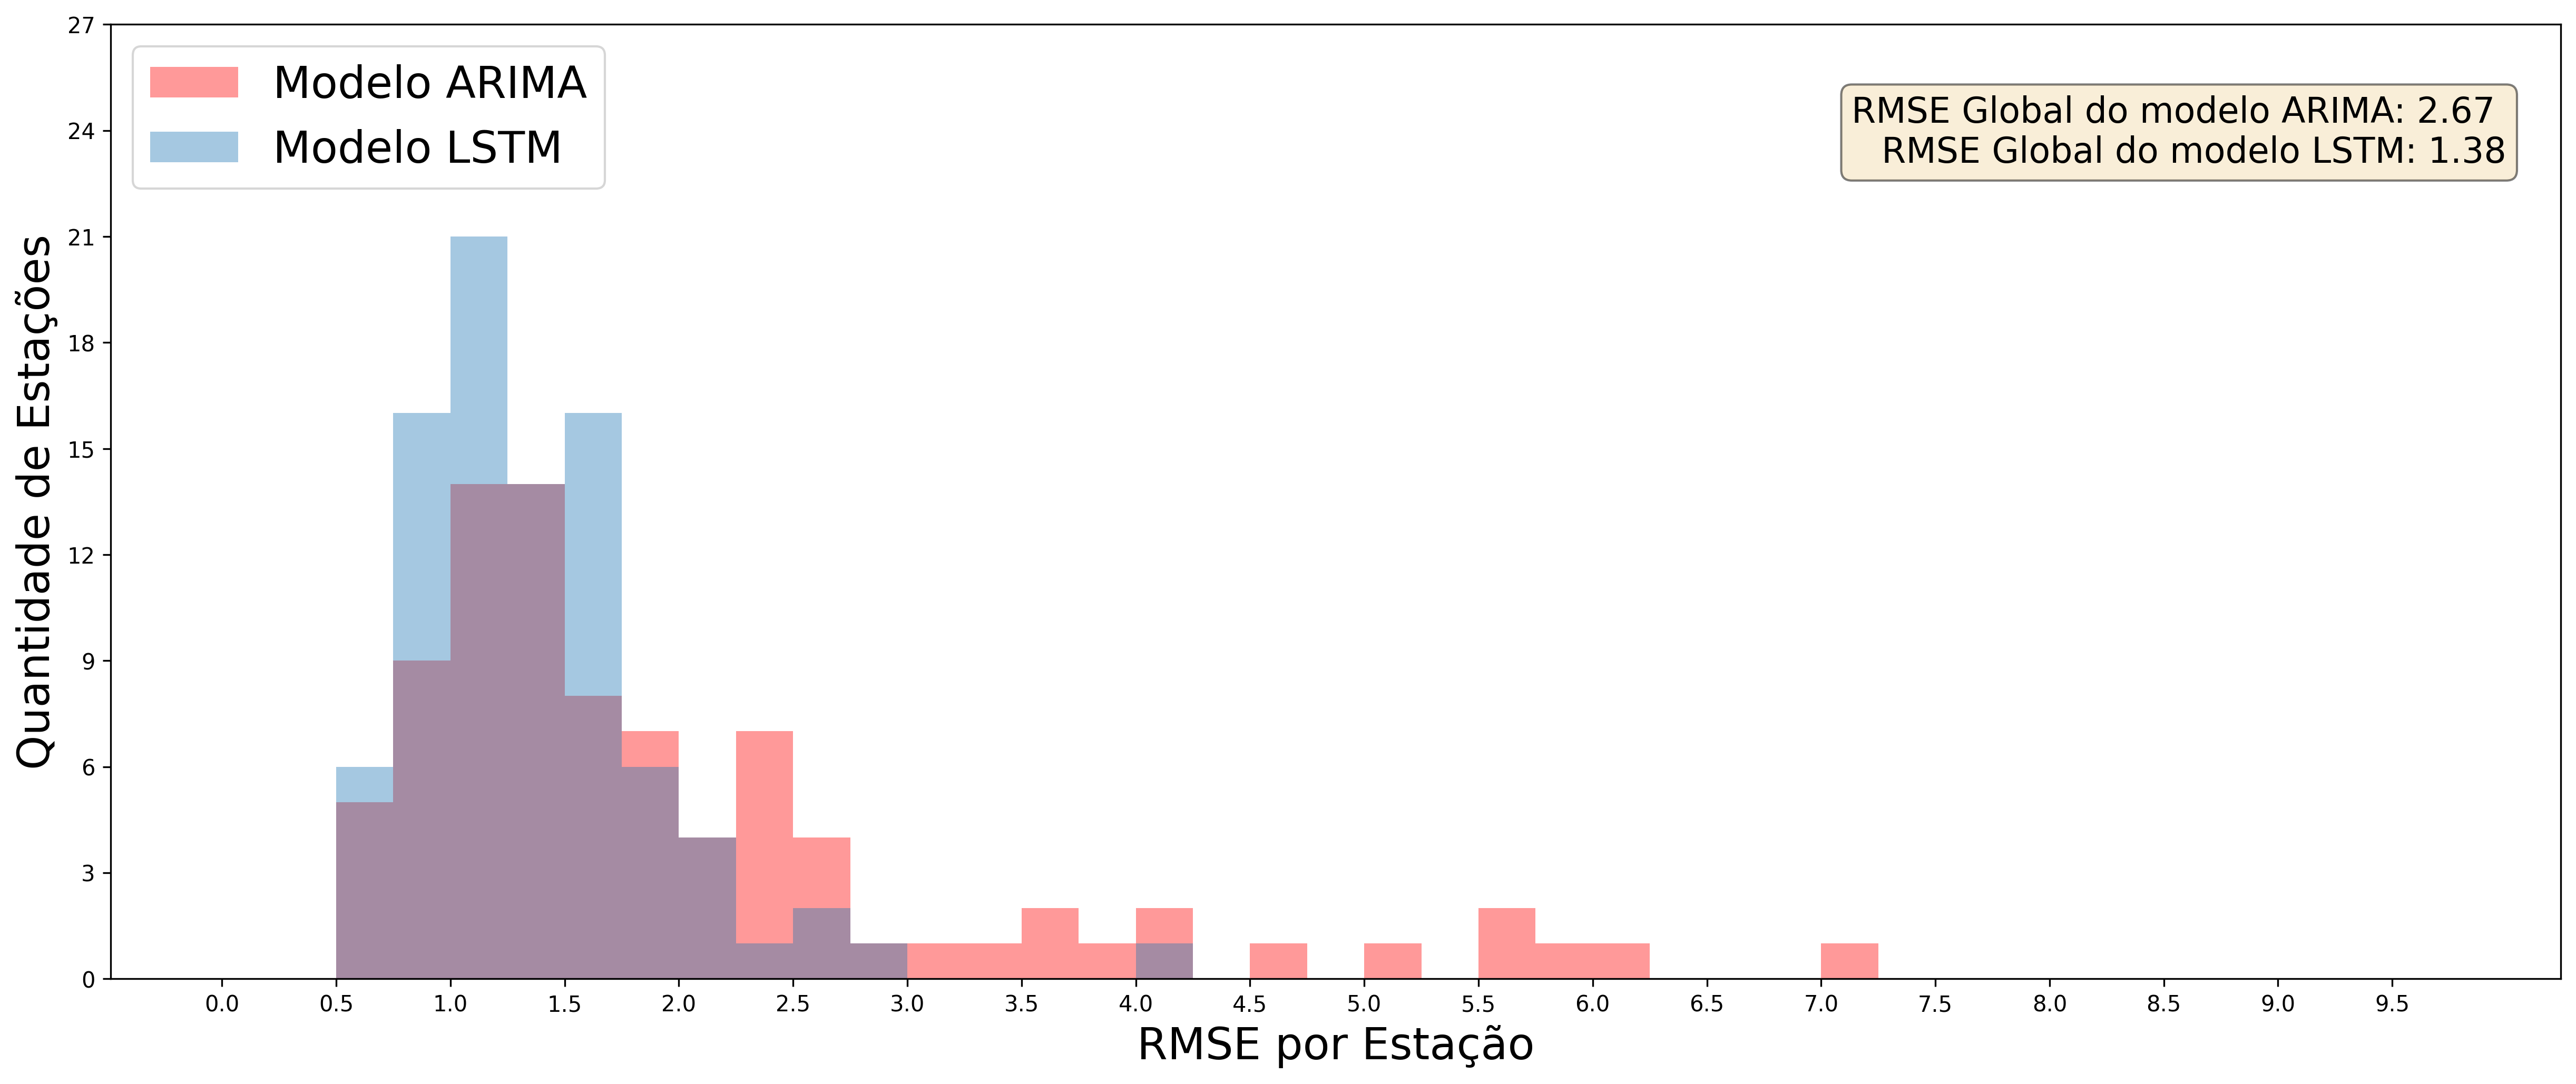
\includegraphics[width=0.9\textwidth]{figuras/comparacao_rmse_arima_lstm_histograma.png}
\end{figure}

\end{frame}


\section{Conclusão e Trabalhos Futuros}

\begin{frame}
\frametitle{Conclusão e Trabalhos Futuros}

\begin{itemize}
   	\item Modelos ARIMA são um dos métodos mais antigos e populares de previsão de séries temporais, conseguem obter bons resultados, mas possuem grande dependência em sua parametrização, o que dificulta sua operacionalização; 
   	\item Modelos baseados em RNNs, como a LSTM, possuem a capacidade de trabalhar com longas séries temporais e, em geral, possuem melhor generalização que modelos clássicos de ML, porém necessitam de grandes conjuntos de dados para o treinamento;  
	\item A utilização de outras variáveis, como a precipitação, umidade relatividade do ar, pressão atmosférica, radiação solar global  e outras, podem ser utilizadas em trabalhos futuros para ajudar na previsão da temperatura do ar, já que muitas dessas variáveis são correlacionadas.  
\end{itemize}
\end{frame}

% % ----------------- NOVO SLIDE --------------------------------
% \section{Referências}

% \begin{frame}[allowframebreaks]{Referências}
% 	\bibliography{referencias}
% \end{frame}

% ----------------- NOVO SLIDE --------------------------------

\begin{frame}
	\begin{columns}
		\begin{column}{3cm}
			
\includegraphics[height=3cm]{figuras/logo.png}
		\end{column}
		\begin{column}{7cm}
			\begin{flushright}
				\centering
				\vskip 0.5cm
				\Huge Obrigado!
			\end{flushright}
		\end{column}
	\end{columns}
\end{frame}


% ----------------- FIM DO DOCUMENTO -----------------------------------------
\end{document}
